% !TEX root = ../thesis.tex

\section{Results}
\label{sec:results}

% Results overview
The results of the search for a new heavy boson resonance are considered in terms of exclusion limits for the benchmark signal models described in this analysis.
These limits are model-independent, and cover spin-0, spin-1, and spin-2 resonances decaying to \WW, \WZ, and \WH.
We also consider the observed $p$-values obtained through a profile likelihood fit.

\subsection{Exclusion Limits}

% Asymptotic limits
The exclusion limits obtained for the analysis are asymptotic frequentist limits for the production cross section times the branching ratio for each signal model.
These limits are obtained by using an asymptotic approximation of the distributions for a test statistic $\tilde{q}_\mu$ that is based on a profile likelihood ratio under signal and background hypotheses with signal strength $\mu$, where $\mu=0$ is the background-only model and $\mu=1$ is the nominal signal model~\cite{Cowan_2011}.

% Obtaining limits
The test statistic used is
\begin{equation}
  \tilde{q}_\mu=\begin{cases}
    -2\ln\tilde{\lambda}(\mu) & \hat{\mu}\leq\mu,\\
    0 & \hat{\mu}>\mu,
  \end{cases}
\end{equation}
where the likelihood ratio $\tilde{\lambda}(\mu)$ is defined by
\begin{equation}
  \tilde{\lambda}(\mu)=\begin{cases}
    \frac{\mathcal{L}(\mu,\hat{\hat{\vb*{\theta}}}(\mu))}{\mathcal{L}(\hat{\mu},\hat{\vb*{\theta}})} & \hat{\mu}\geq0,\\
    \frac{\mathcal{L}(\mu,\hat{\hat{\vb*{\theta}}}(\mu))}{\mathcal{L}(0,\hat{\hat{\vb*{\theta}}}(0))} & \hat{\mu}<0,
  \end{cases}
\end{equation}
with $\hat{\hat{\vb*{\theta}}}$ corresponding to the conditional maximum likelihood estimators of $\vb*{\theta}$.
After finding the observed test statistic $\tilde{q}_{\mu,\mathrm{obs}}$, we generate toy MCs to construct the pdfs for $\tilde{q}_\mu$ for both signal and background-only experiments.
This is used to find the $p$-value for the signal $p_\mu$, given by
\begin{equation}
  p_\mu=\int_{\tilde{q}_{\mu,\mathrm{obs}}}^\infty f(\tilde{q}_\mu|\mu,\hat{\hat{\vb*{\theta}}}(\mu,\mathrm{obs}))\dd{\tilde{q}_\mu},
\end{equation}
where $f(\tilde{q}_\mu|\mu,\hat{\hat{\vb*{\theta}}}(\mu,\mathrm{obs}))$ is the signal+background pdf for $\tilde{q}_\mu$, and $\hat{\hat{\vb*{\theta}}}(\mu,\mathrm{obs})$ is the conditional maximum likelihood estimate based on the observed data.
The confidence-level (CL) upper limit $CL_s$ is obtained by computing the $p$-value for the background-only hypothesis, defined by
\begin{equation}
  p_b=1-\int_{\tilde{q}_{\mu,\mathrm{obs}}}^\infty f(\tilde{q}_\mu|0,\hat{\hat{\vb*{\theta}}}(0,\mathrm{obs}))\dd{\tilde{q}_\mu},
\end{equation}
with $f(\tilde{q}_\mu|0,\hat{\hat{\vb*{\theta}}}(0,\mathrm{obs}))$ corresponding to the background-only pdf for $\tilde{q}_\mu$.
We then define the $CL_s$ upper limit as
\begin{equation}
  CL_s=\frac{p_\mu}{1-p_b}.
\end{equation}

% Observed limits
We derive 95\% CL upper limits on the resonance production cross section times branching ratio to \WW, \WZ, or \WH as a function of the mass hypothesis \MX for a narrow resonance, and compare them to expected cross sections from the benchmark models where available.
We also obtain the corresponding local $p$-values as a function of \MX.
The resulting limits and local $p$-values are shown in figures~\ref{fig:limits_pvalue_spin0}, \ref{fig:limits_pvalue_spin1_neut}, \ref{fig:limits_pvalue_spin1_char}, and \ref{fig:limits_pvalue_spin2} for the spin-0, spin-1, and spin-2 signal models.
These limits are obtained for the combination of all 24 search categories, showing the observed and median expected limits with the 68\% and 95\% expected bands.

% Observed excesses
No significant excess is observed for the \ggF and \VBF spin-0 and spin-2 signals, nor for the \DY spin-1 signals.
However, a possible excess is observed for the \VBF spin-1 signals for both the neutral and charged signal models.
The excesses for both signal models occur at $1\unit{TeV}$, with the largest $p$-value occurring in the \VBF\ZprtoWW model with $3.3\sigma$ local significance.
While this warrants further investigation in future analyses, this does not meet the required $5\sigma$ threshold for discovery as of this writing.

\begin{figure}[htbp]
  \centering
  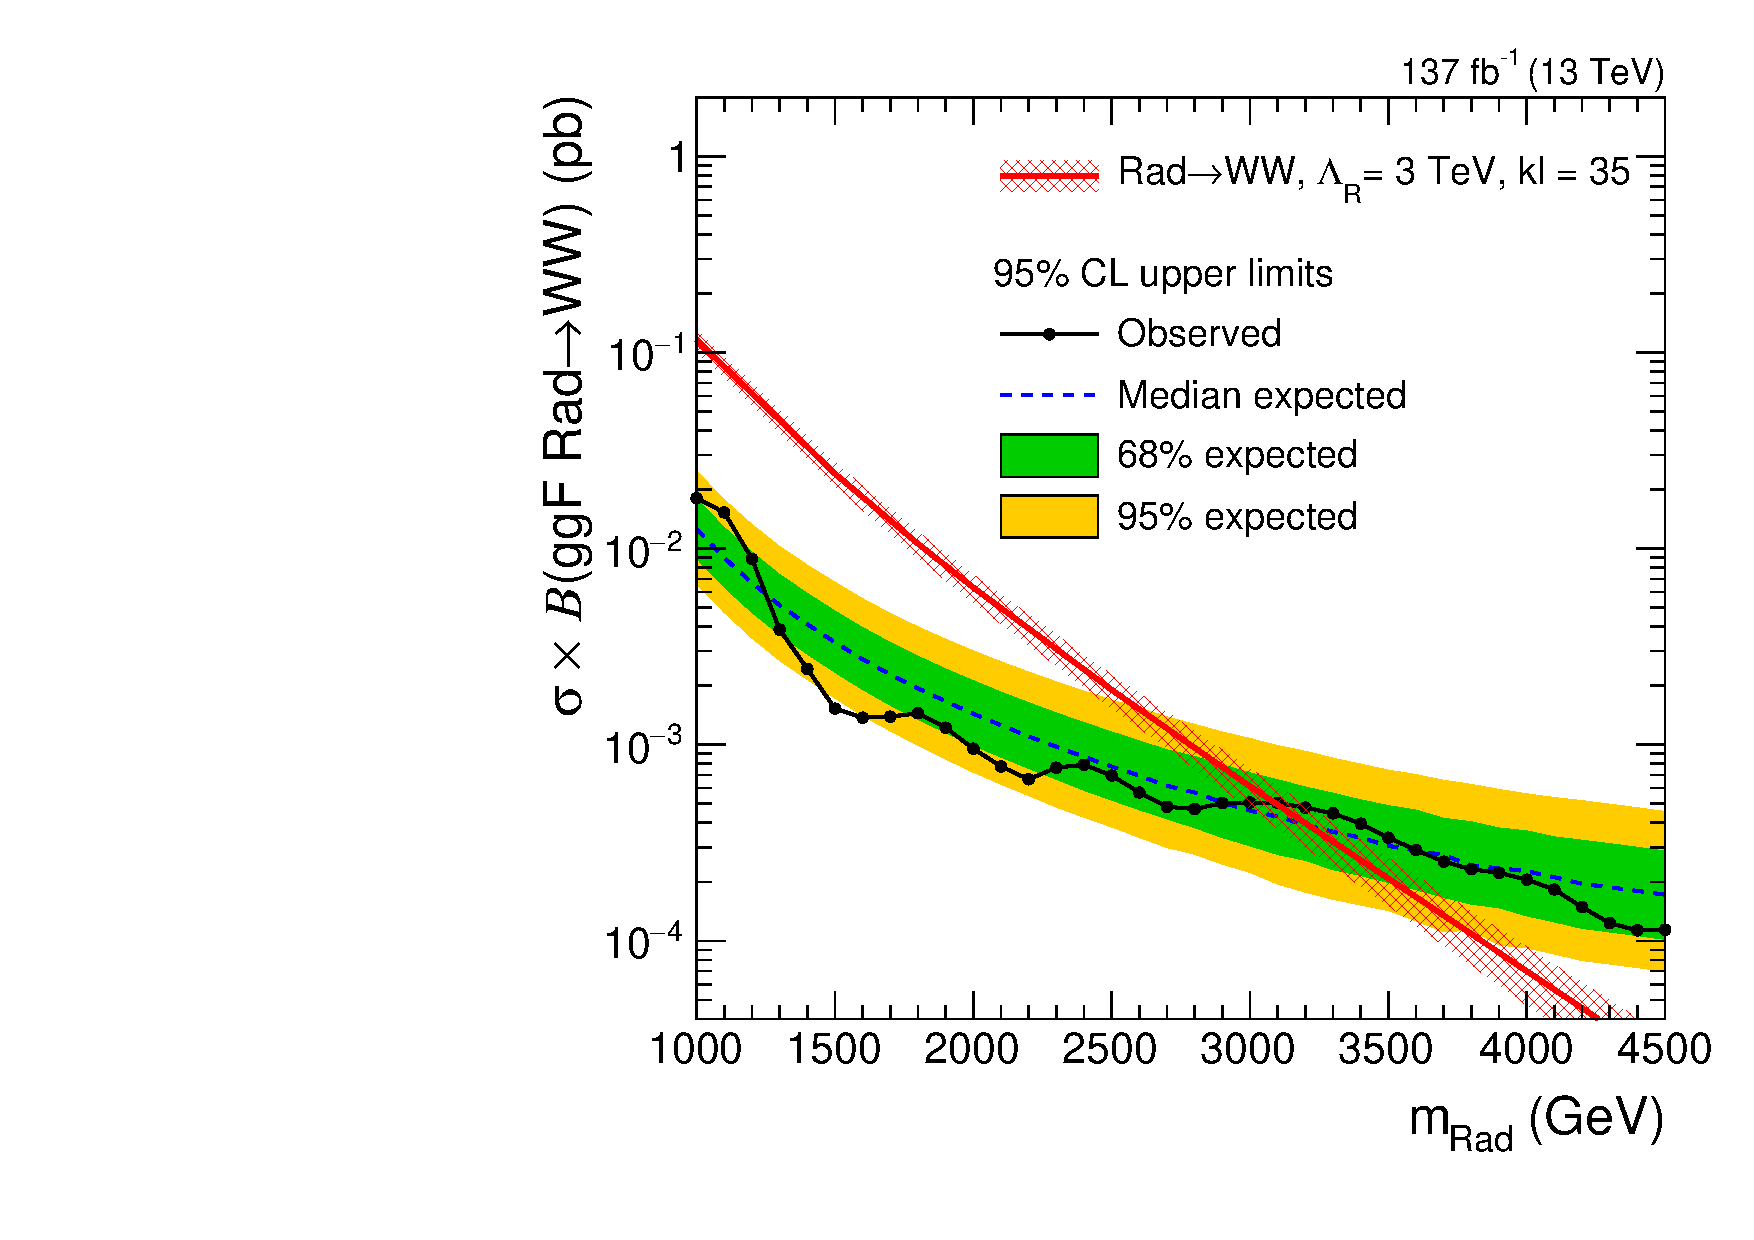
\includegraphics[width=0.33\textwidth]{fig/results/limits_RadToWW.pdf}
  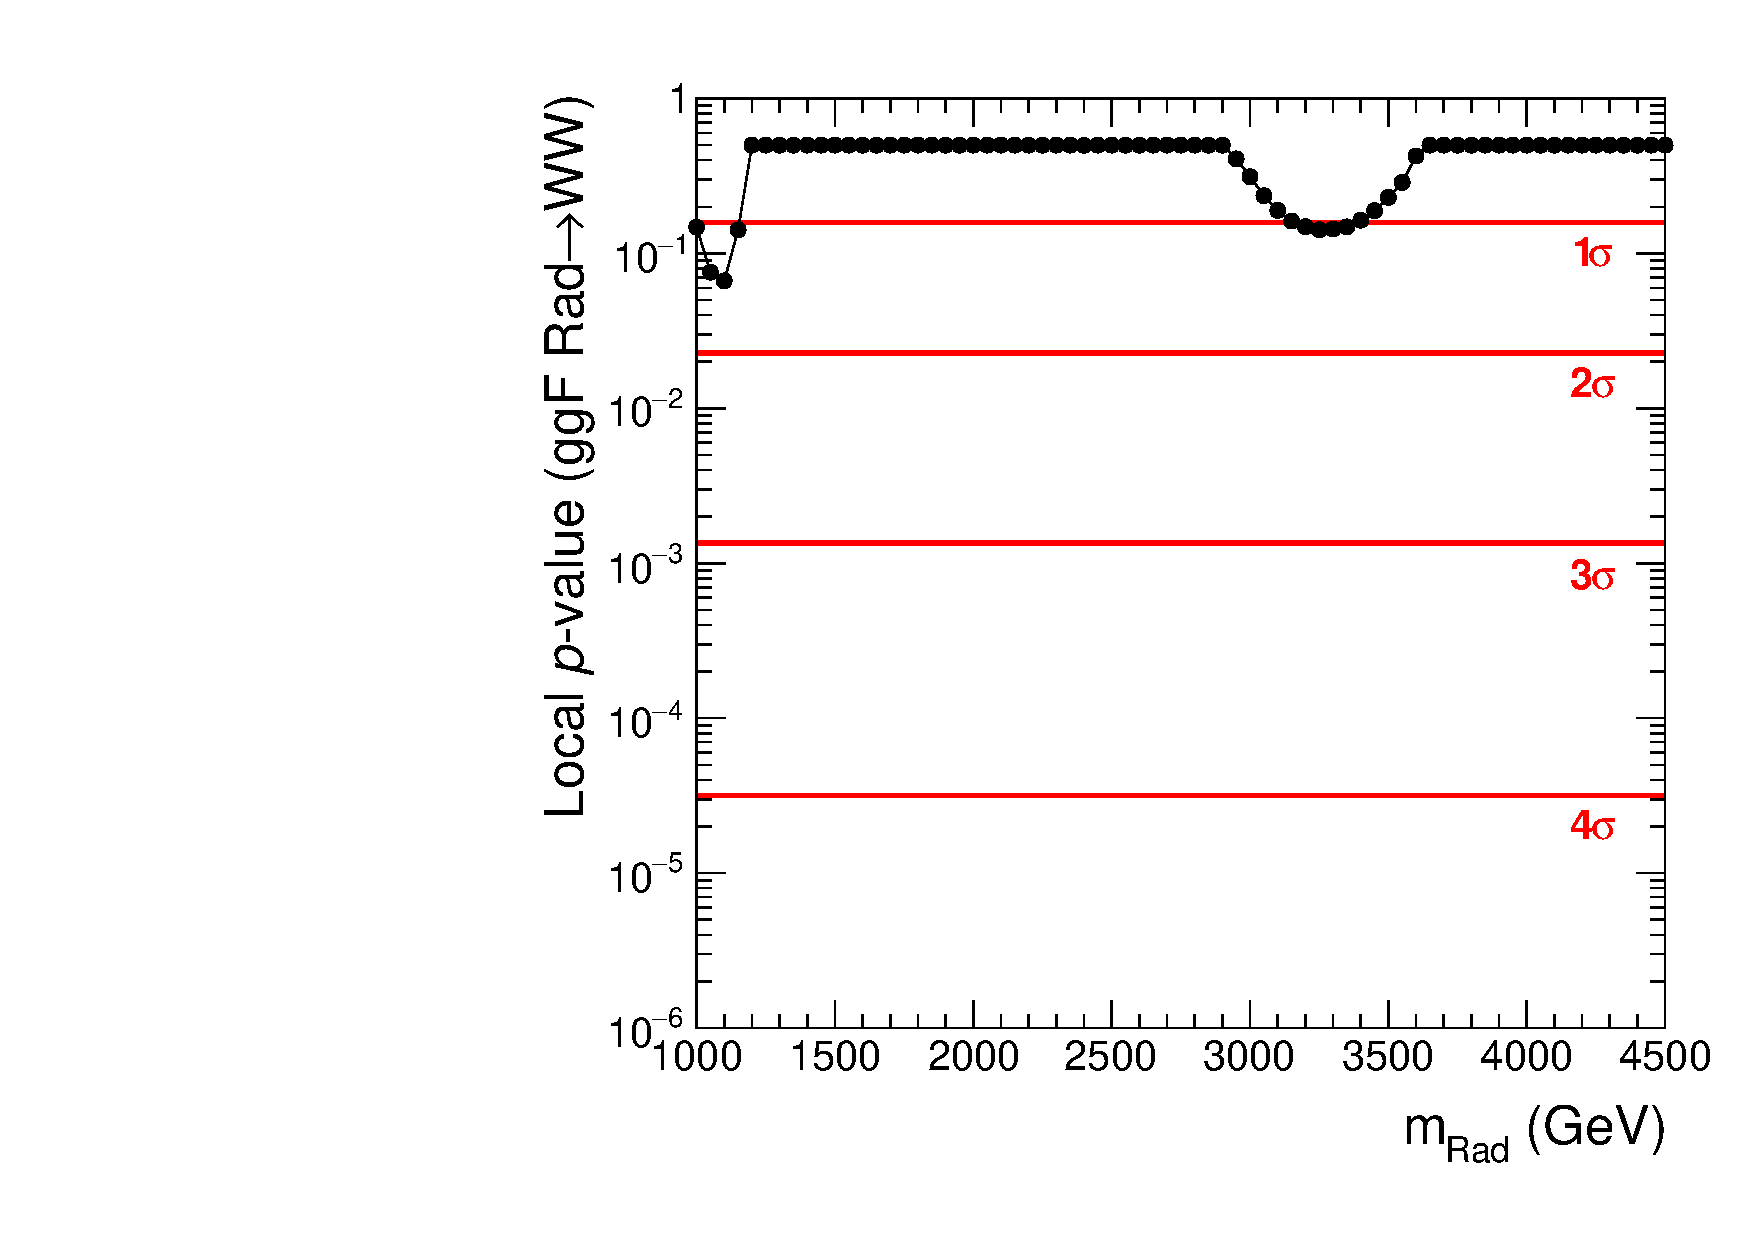
\includegraphics[width=0.33\textwidth]{fig/results/pvalue_RadToWW.pdf}\\
  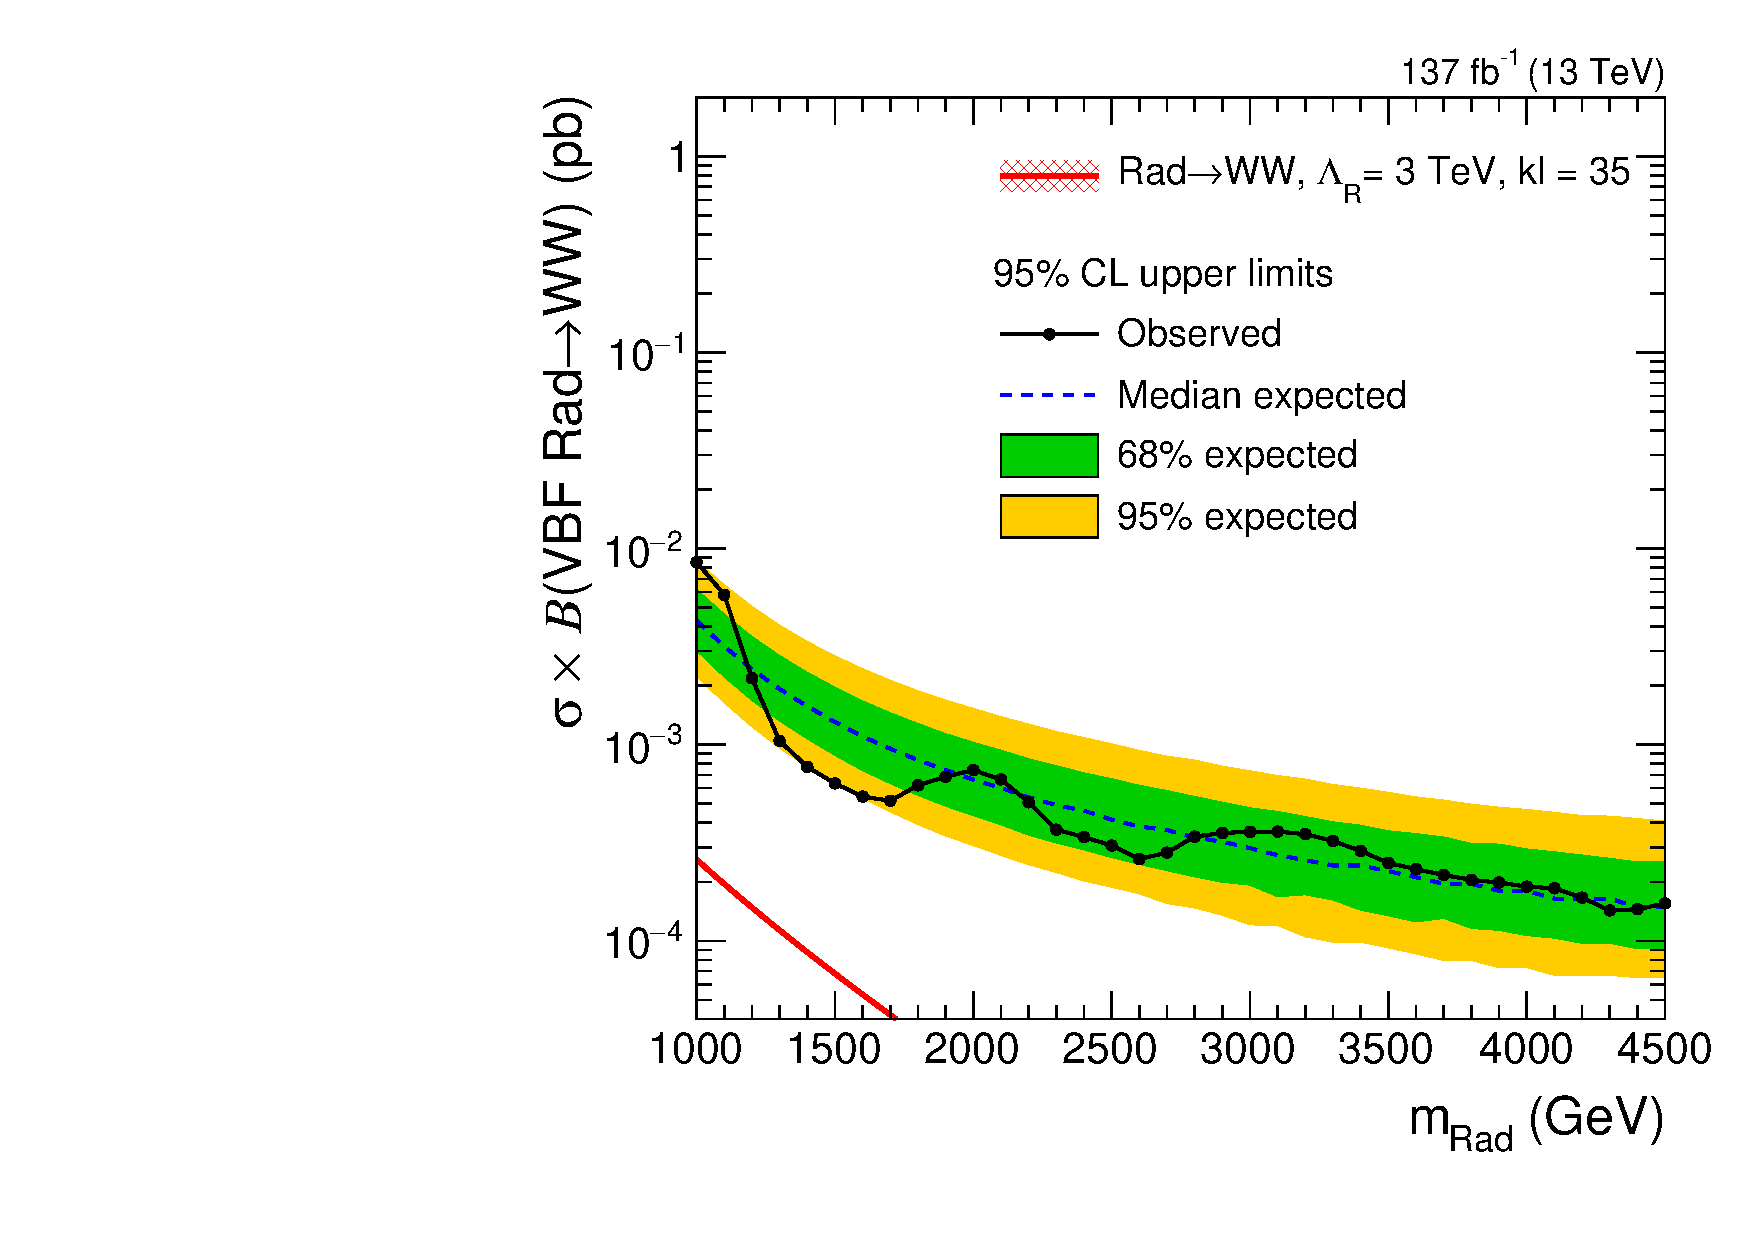
\includegraphics[width=0.33\textwidth]{fig/results/limits_VBFRadToWW.pdf}
  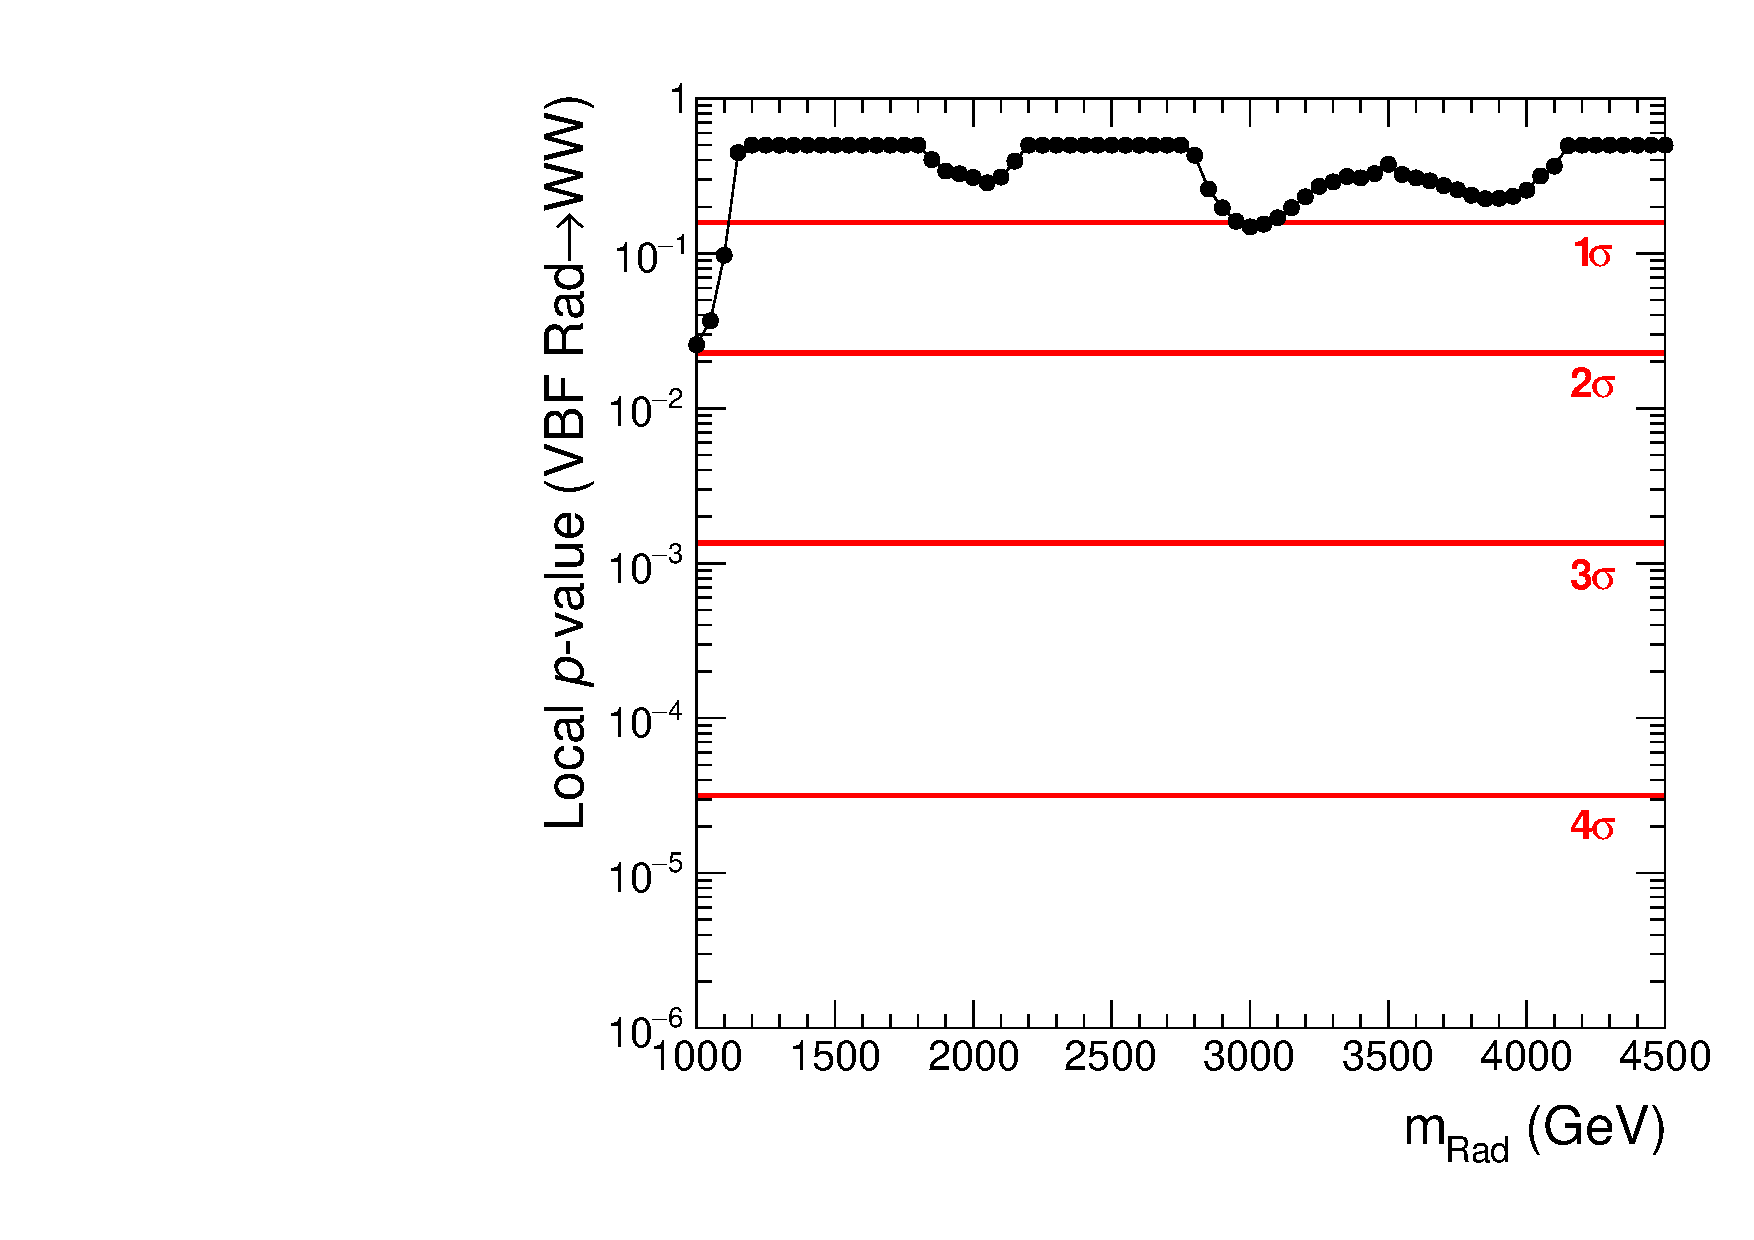
\includegraphics[width=0.33\textwidth]{fig/results/pvalue_VBFRadToWW.pdf}
  \caption{
    Exclusion limits on the product of the production cross section with the branching ratio (left) and $p$-values (right) for a new neutral spin-0 resonance produced via gluon-gluon fusion (top row) or vector boson fusion (bottom row) and decaying to \WW, as a function of the resonance mass hypothesis \MX, compared with the predicted cross sections for a spin-0 bulk radion with $\Lambda_{R}=3\unit{TeV}$ and $kl=35$.
    The signal cross section uncertainties are shown as red cross-hatched bands.
  }
  \label{fig:limits_pvalue_spin0}
\end{figure}

\begin{figure}[htbp]
  \centering
  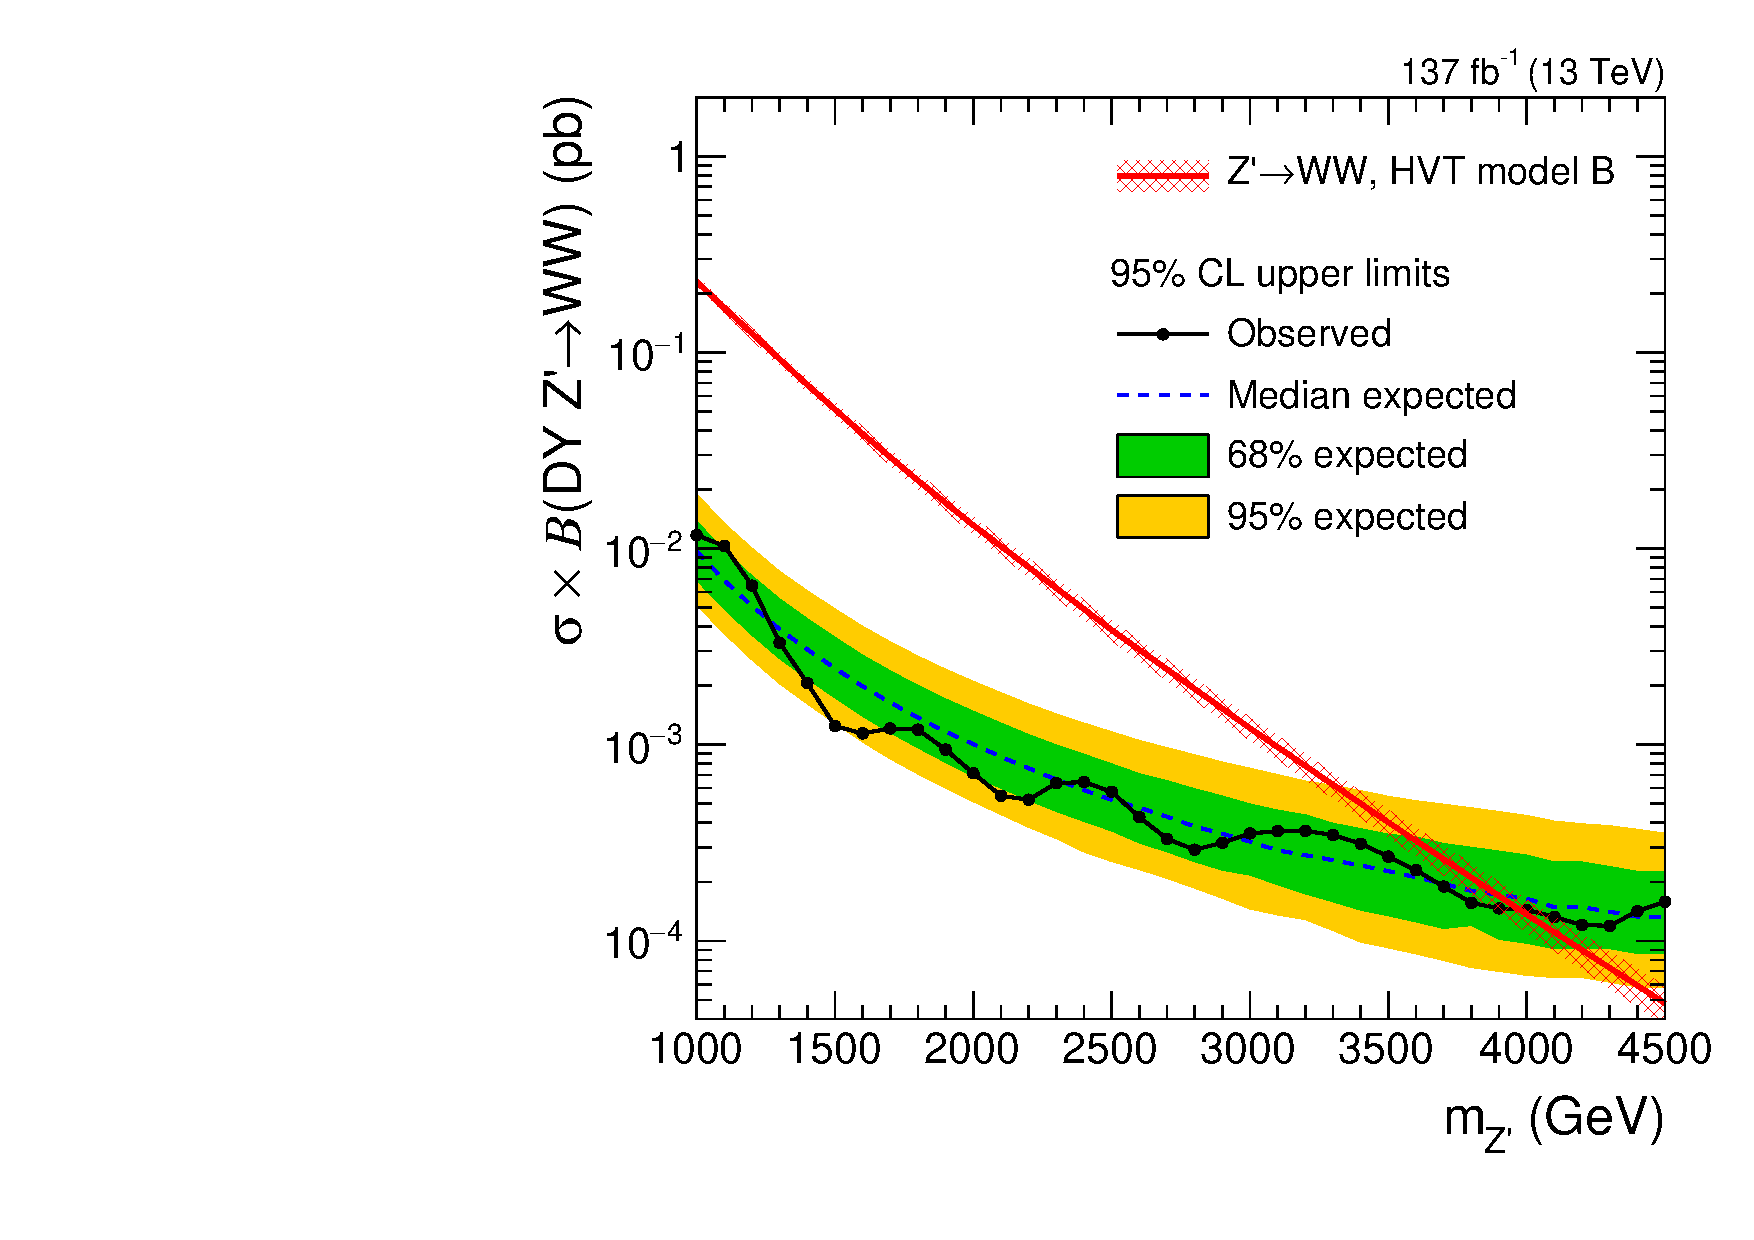
\includegraphics[width=0.33\textwidth]{fig/results/limits_ZprToWW.pdf}
  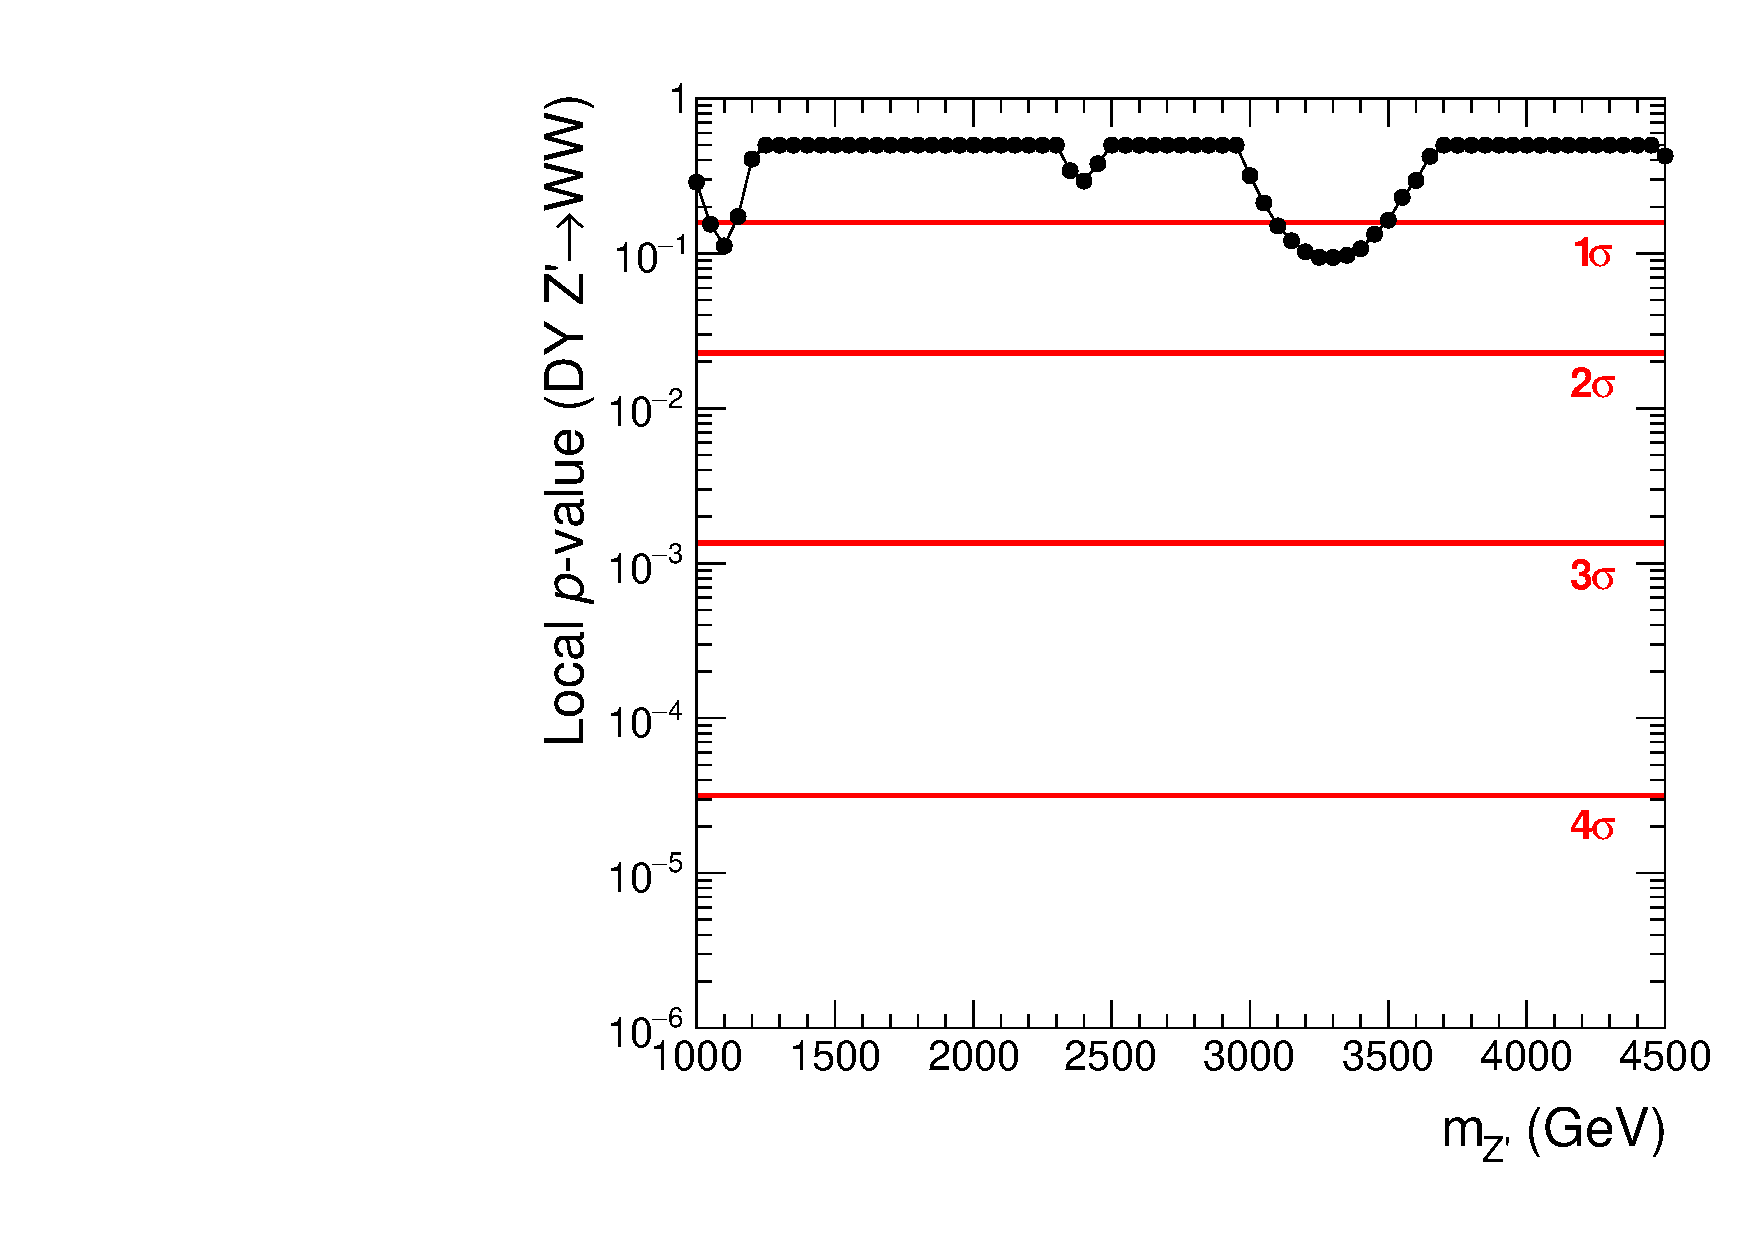
\includegraphics[width=0.33\textwidth]{fig/results/pvalue_ZprToWW.pdf}\\
  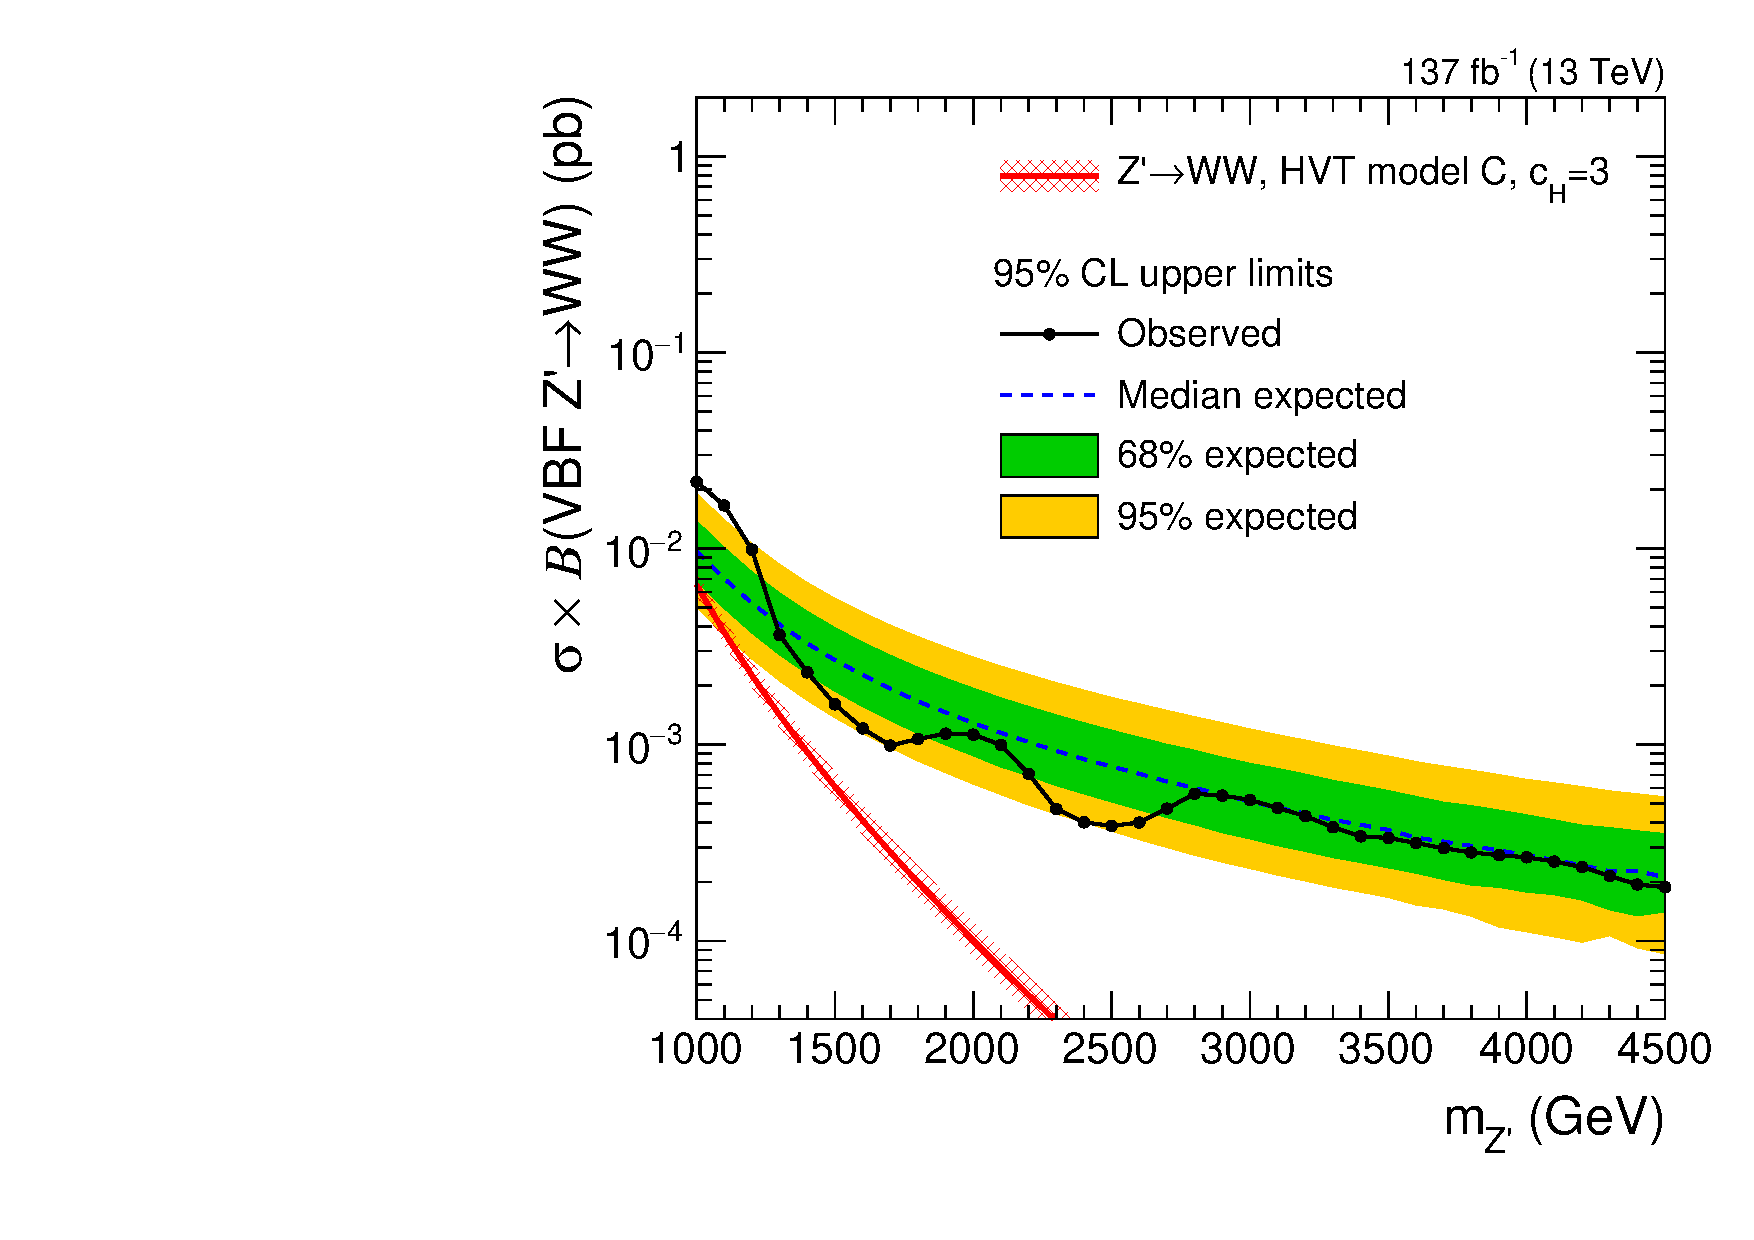
\includegraphics[width=0.33\textwidth]{fig/results/limits_VBFZprToWW.pdf}
  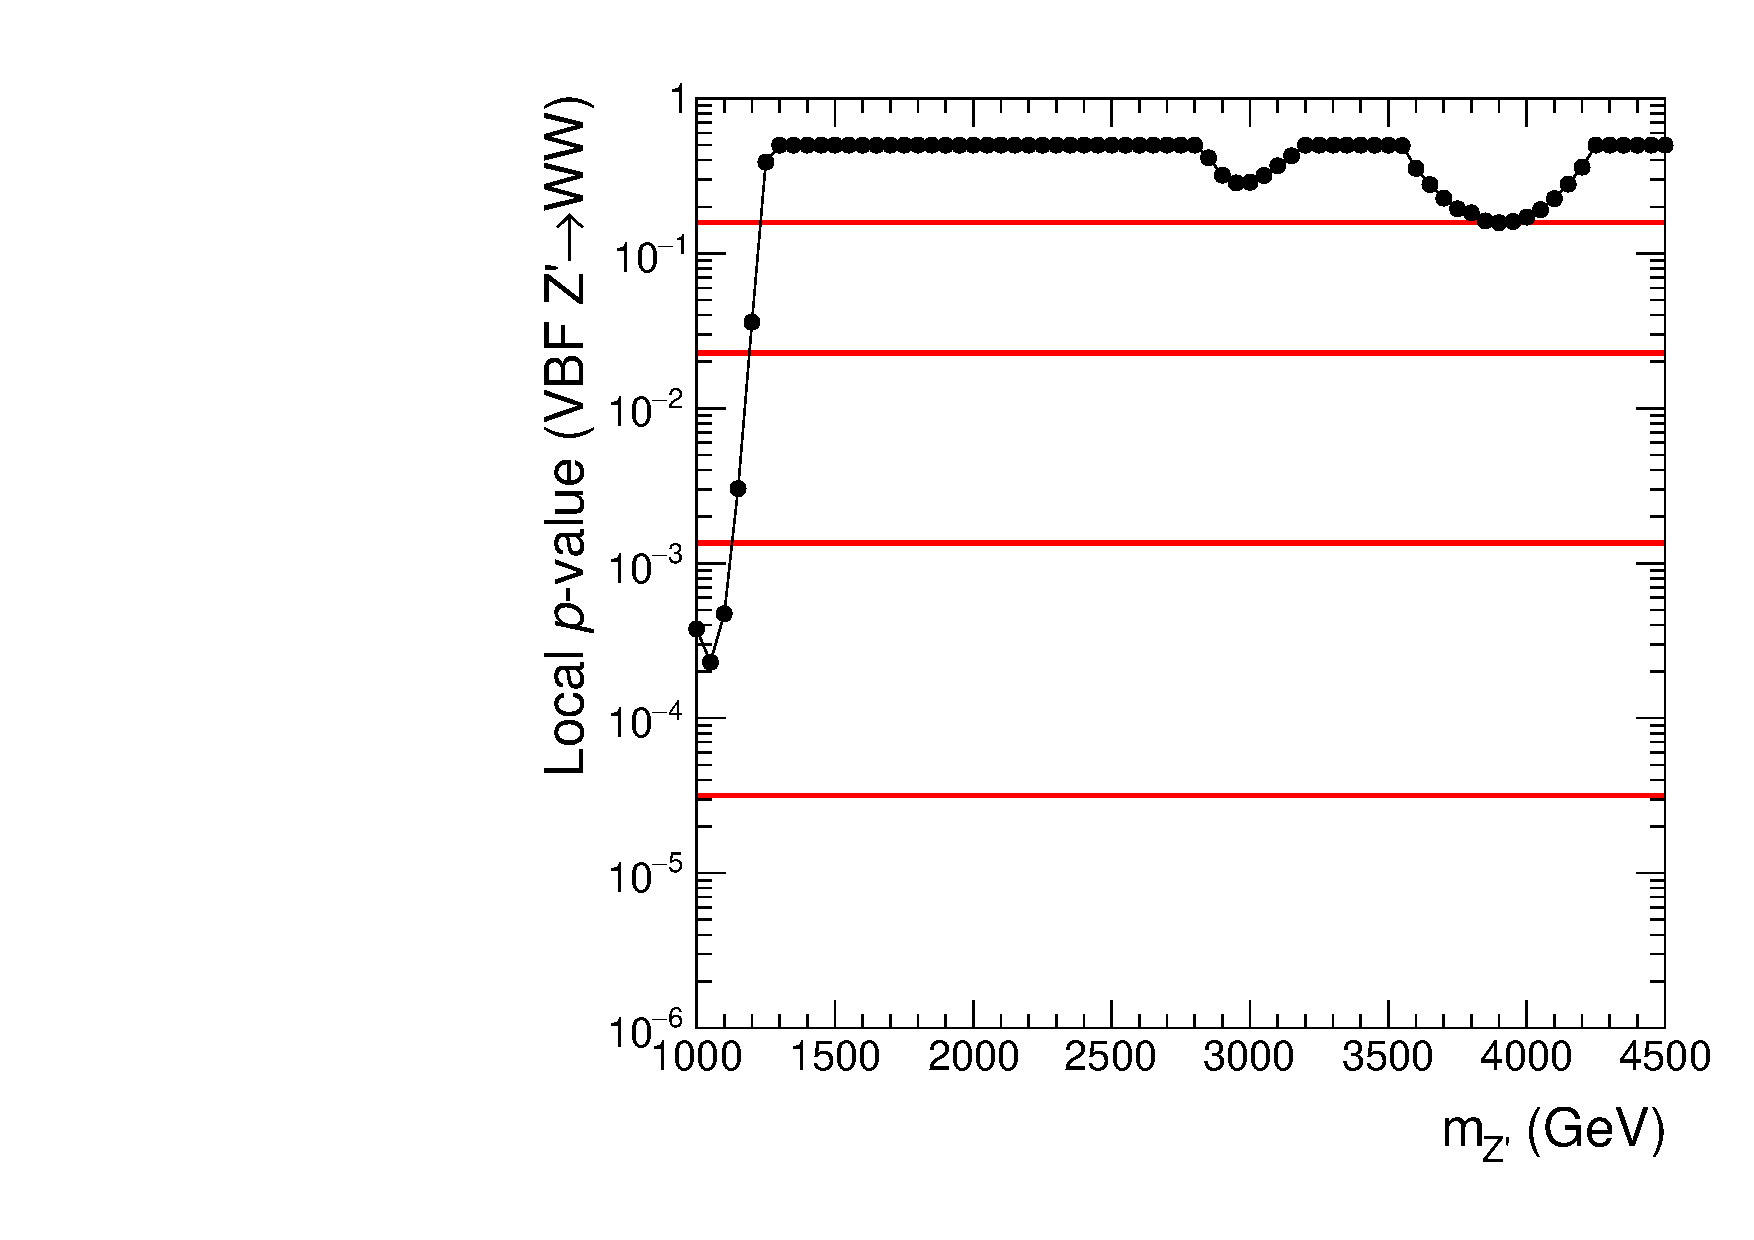
\includegraphics[width=0.33\textwidth]{fig/results/pvalue_VBFZprToWW.pdf}
  \caption{
    Exclusion limits on the product of the production cross section with the branching ratio (left) and $p$-values (right) for a new neutral spin-1 resonance produced via Drell-Yan (top row) or vector boson fusion (bottom row) and decaying to \WW, as a function of the resonance mass hypothesis \MX, compared with the predicted cross sections for a \Zpr from HVT model B (for \DY) or HVT model C with $c_\mathrm{H}=3$ (for \VBF).
    The signal cross section uncertainties are shown as red cross-hatched bands.
  }
  \label{fig:limits_pvalue_spin1_neut}
\end{figure}

\begin{figure}[htbp]
  \centering
  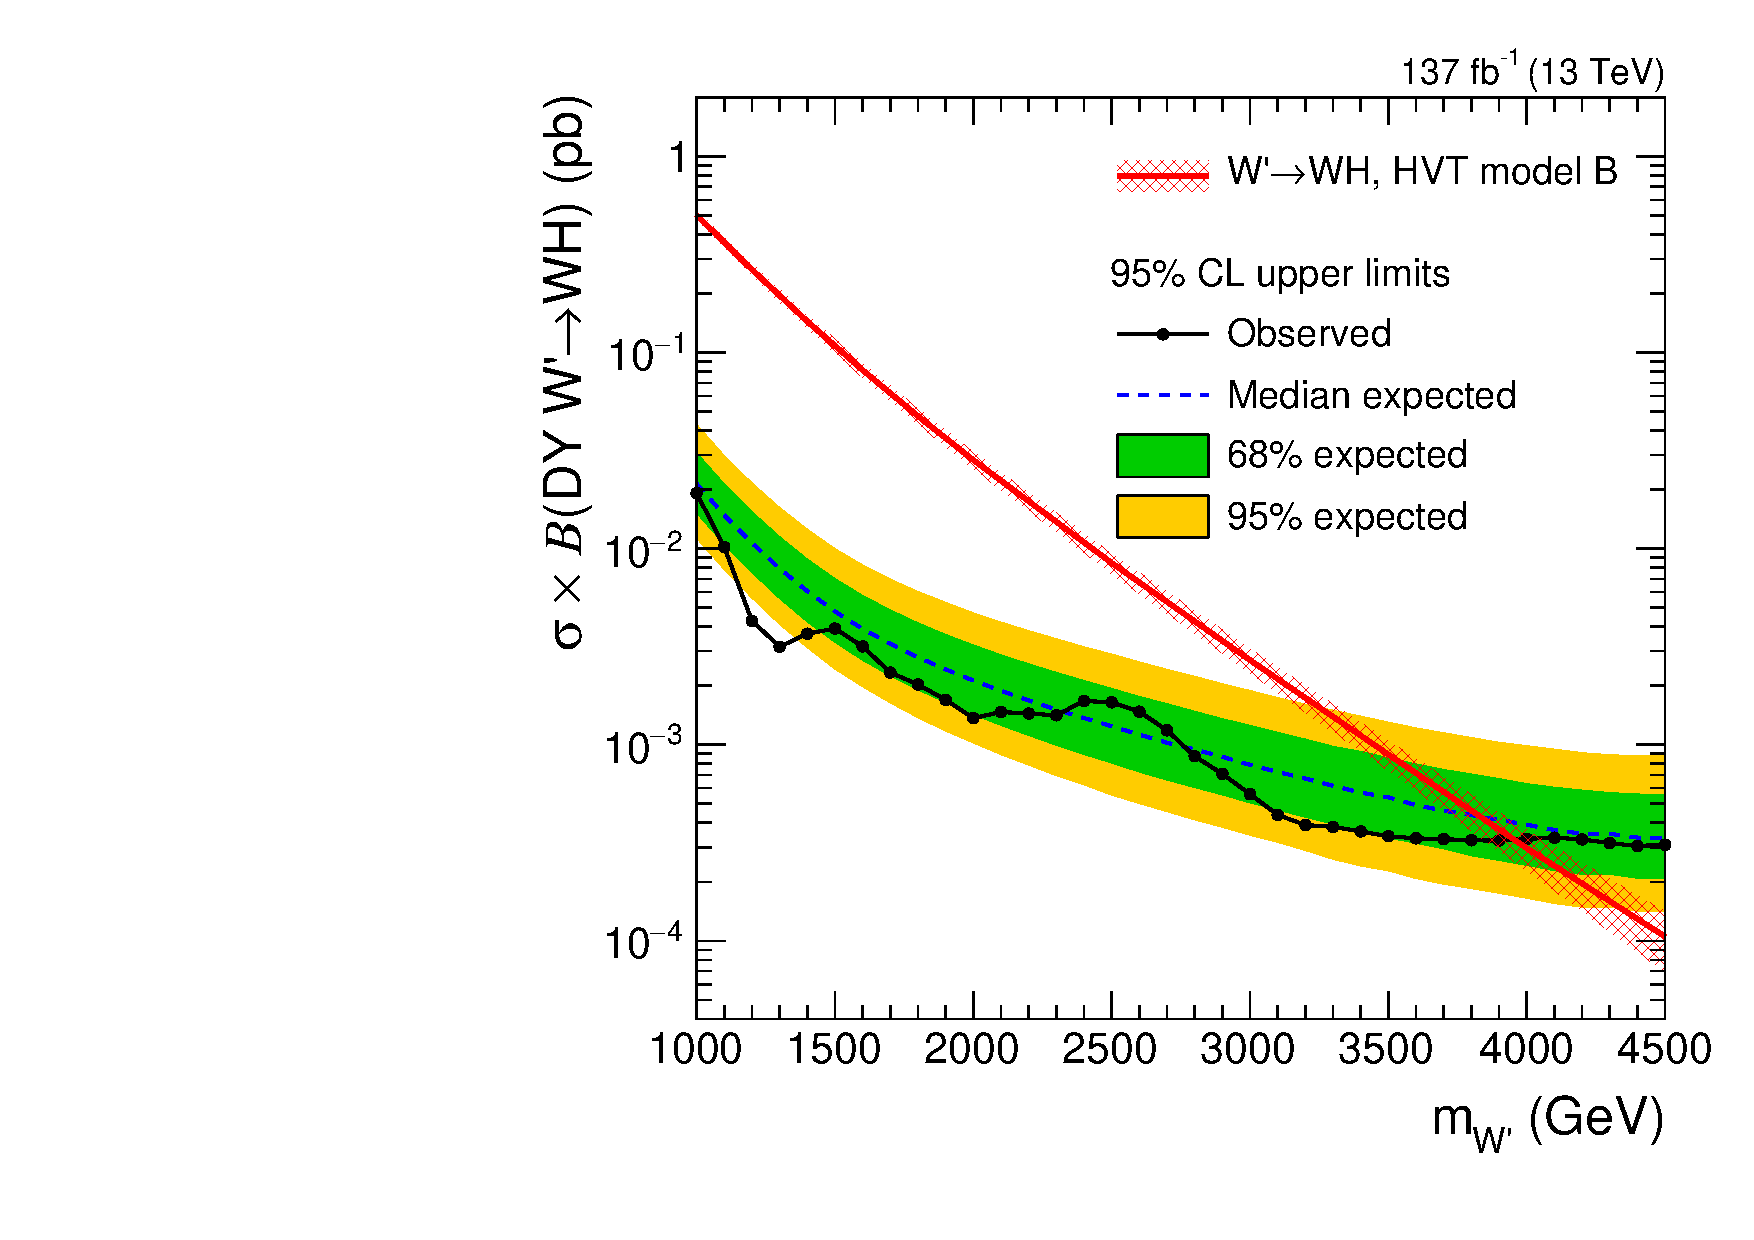
\includegraphics[width=0.33\textwidth]{fig/results/limits_WprToWH.pdf}
  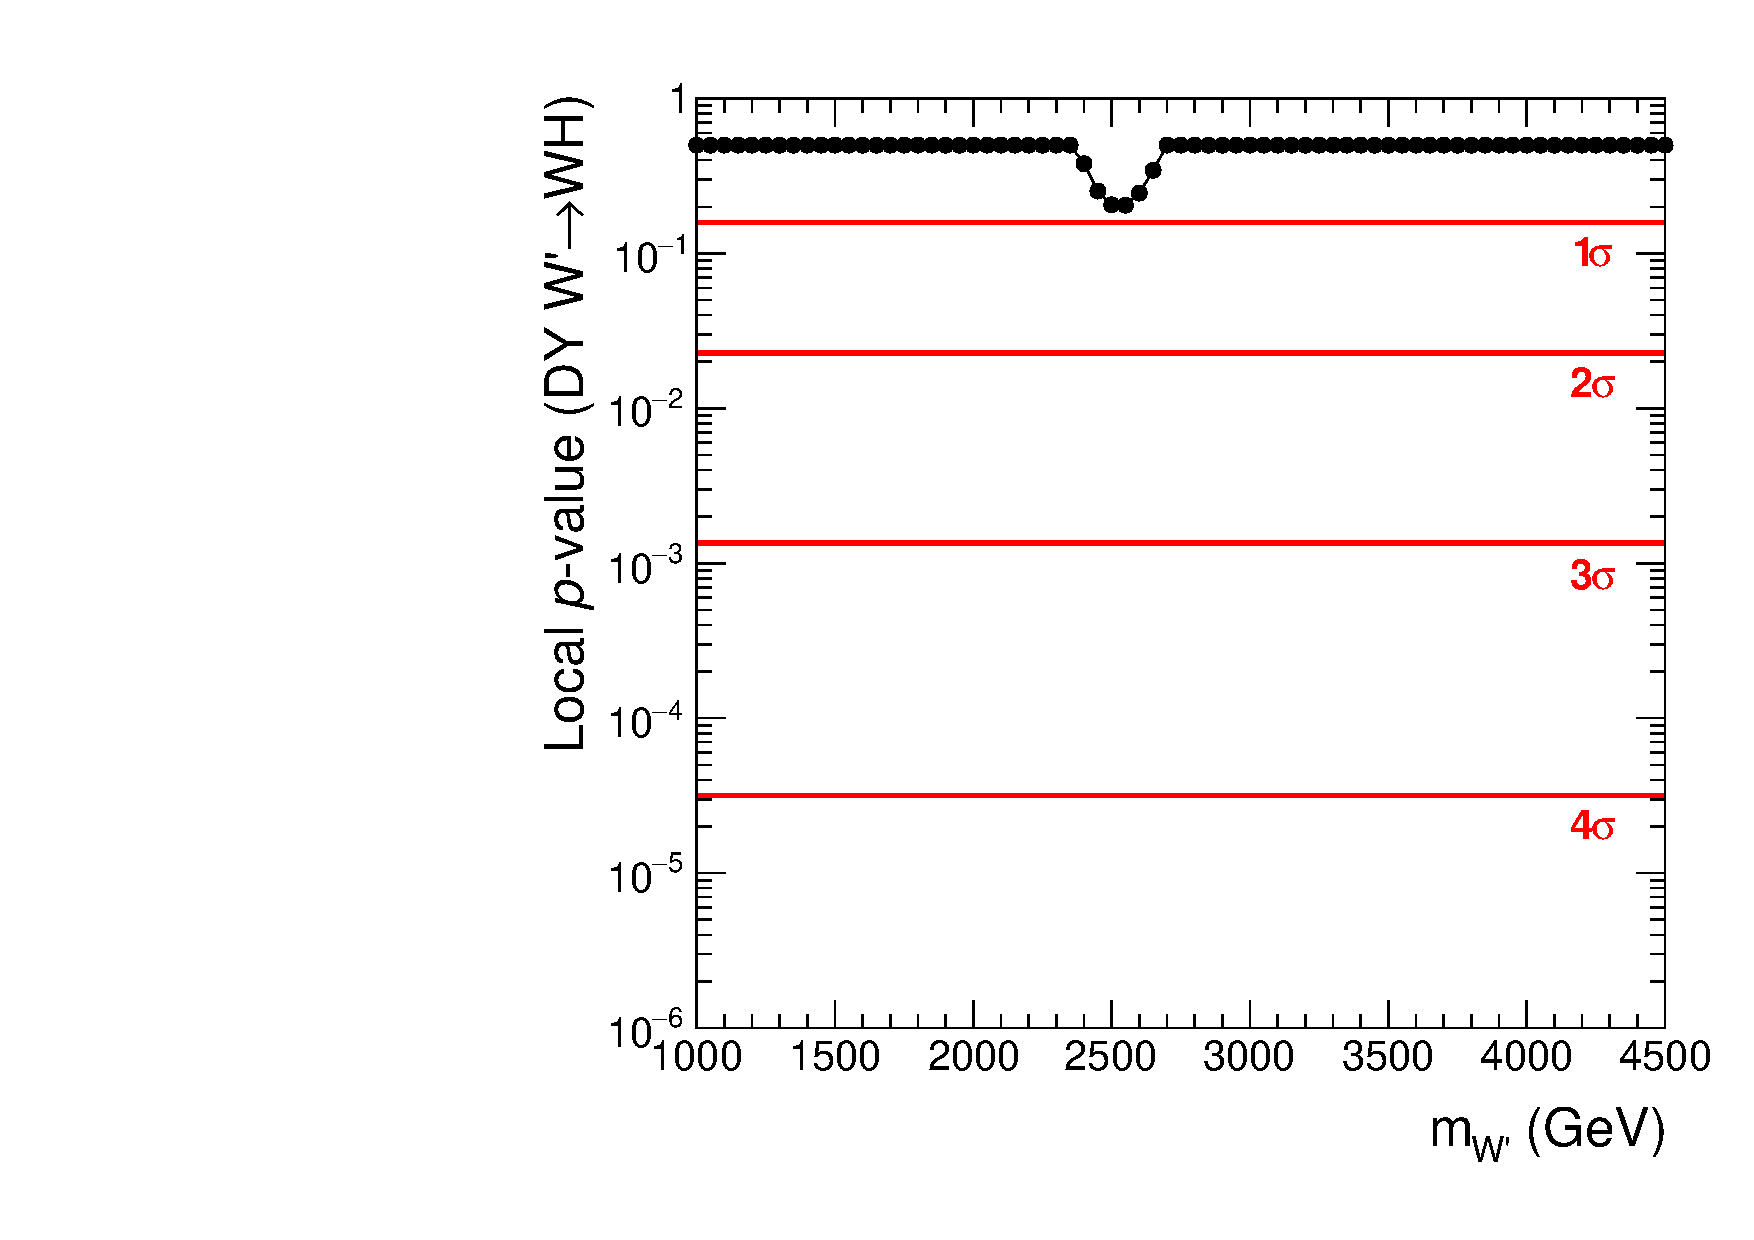
\includegraphics[width=0.33\textwidth]{fig/results/pvalue_WprToWH.pdf}\\
  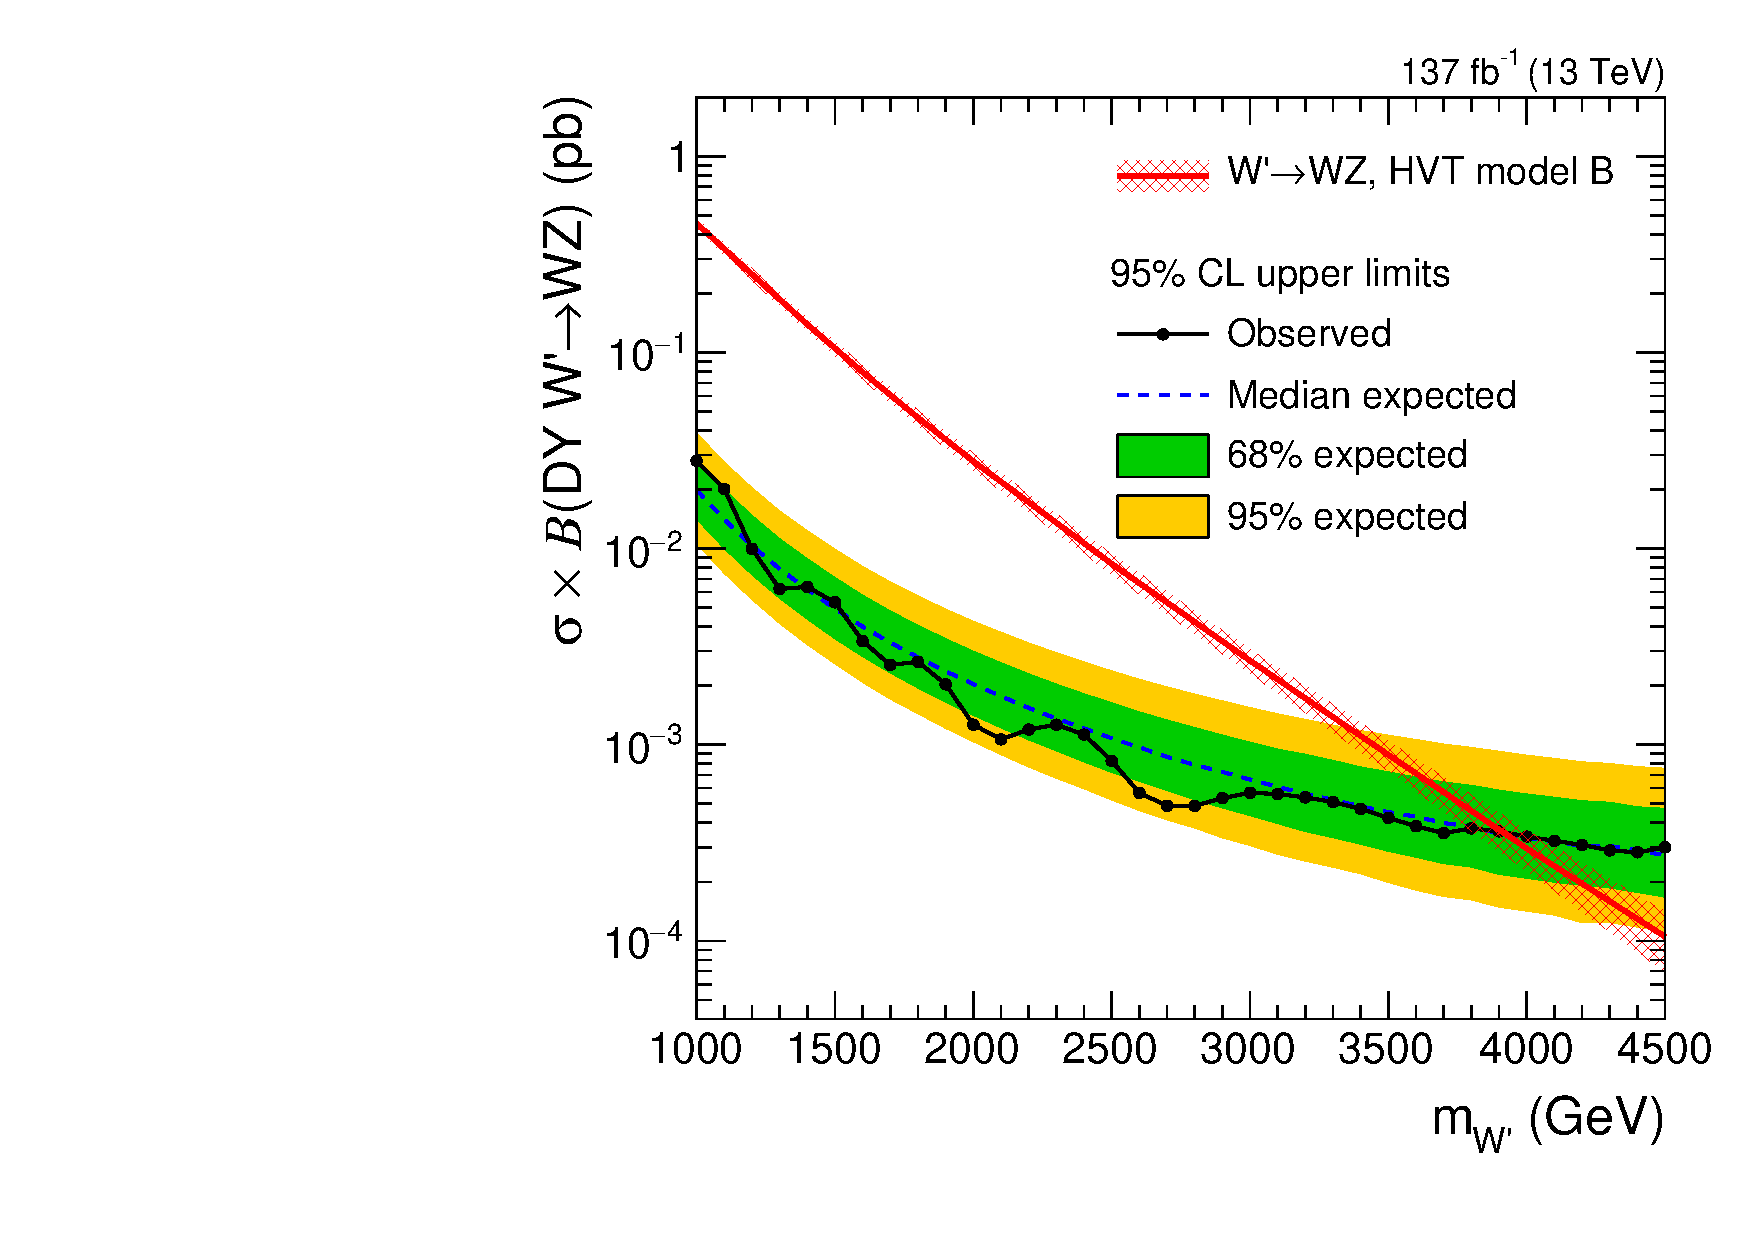
\includegraphics[width=0.33\textwidth]{fig/results/limits_WprToWZ.pdf}
  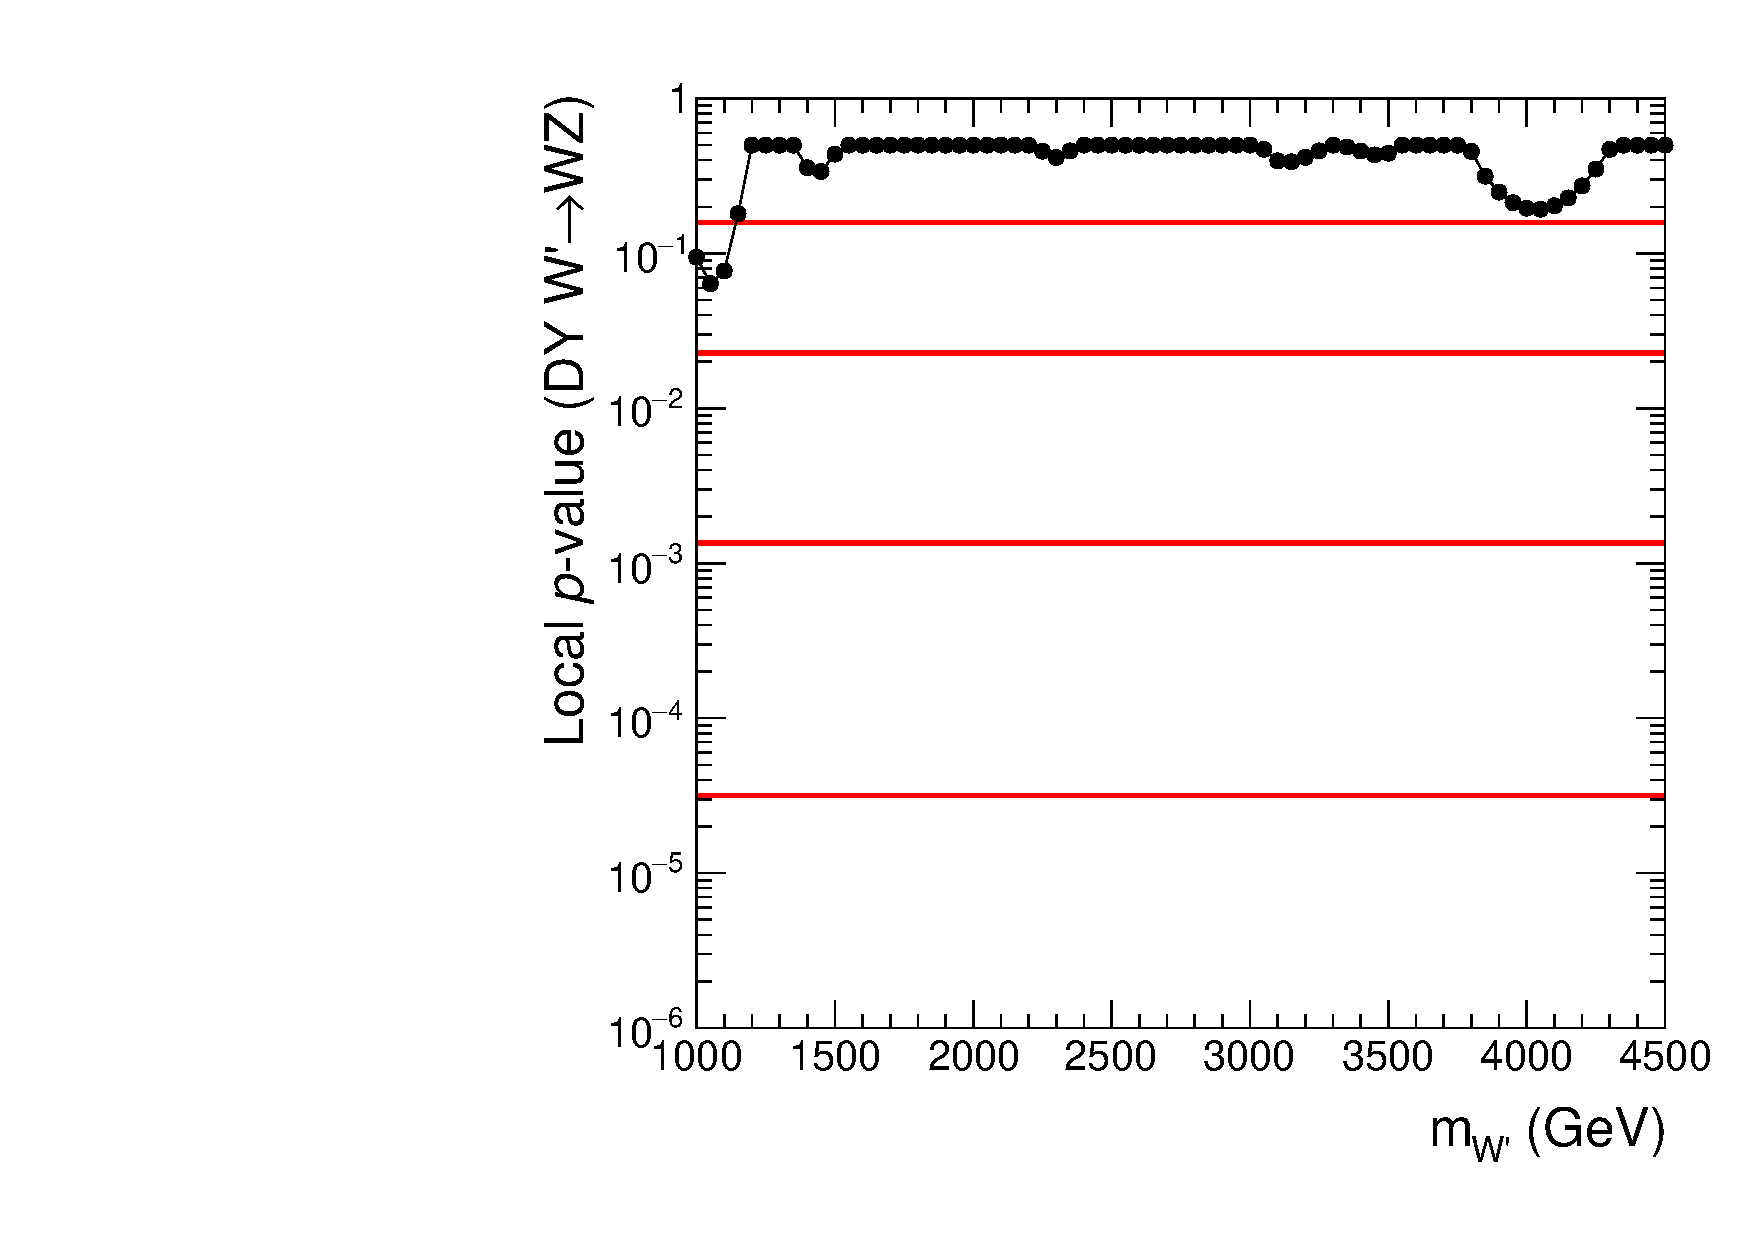
\includegraphics[width=0.33\textwidth]{fig/results/pvalue_WprToWZ.pdf}\\
  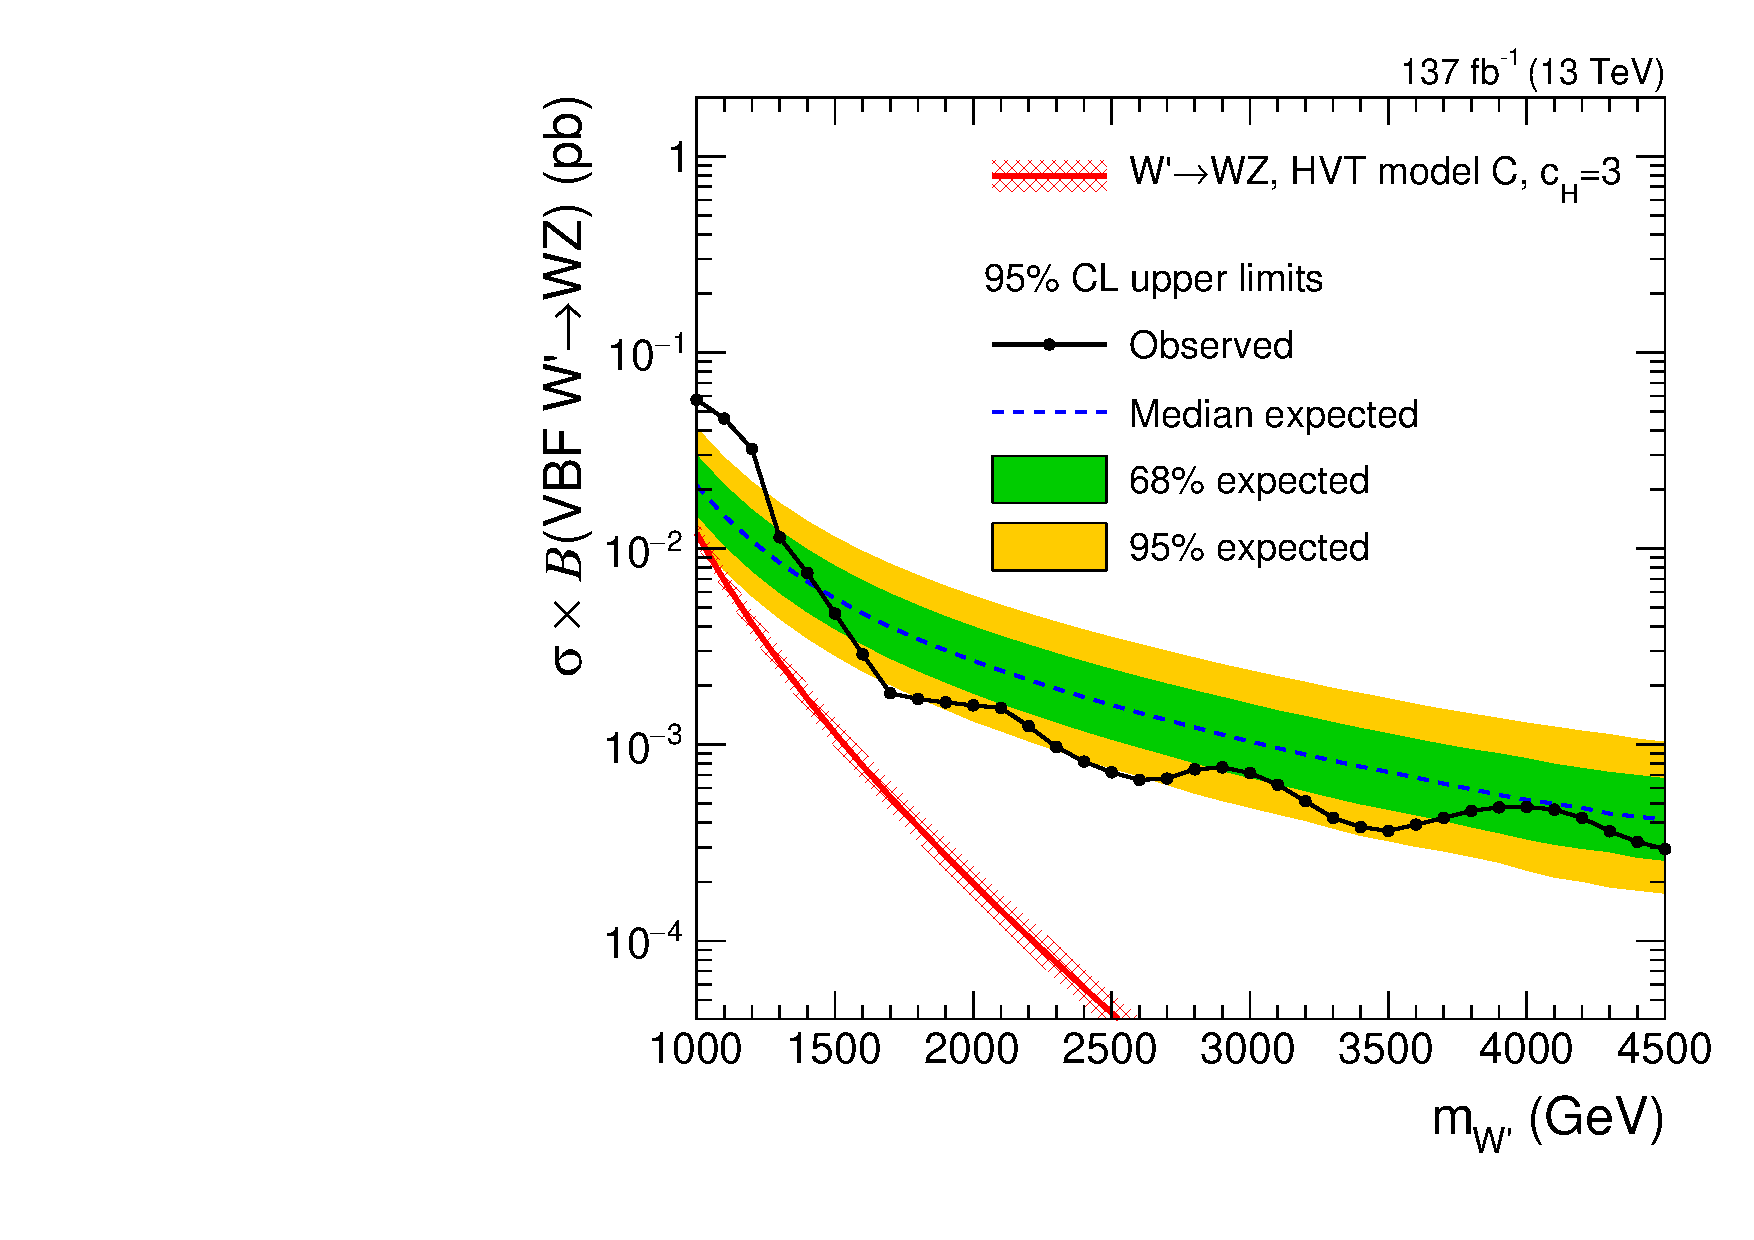
\includegraphics[width=0.33\textwidth]{fig/results/limits_VBFWprToWZ.pdf}
  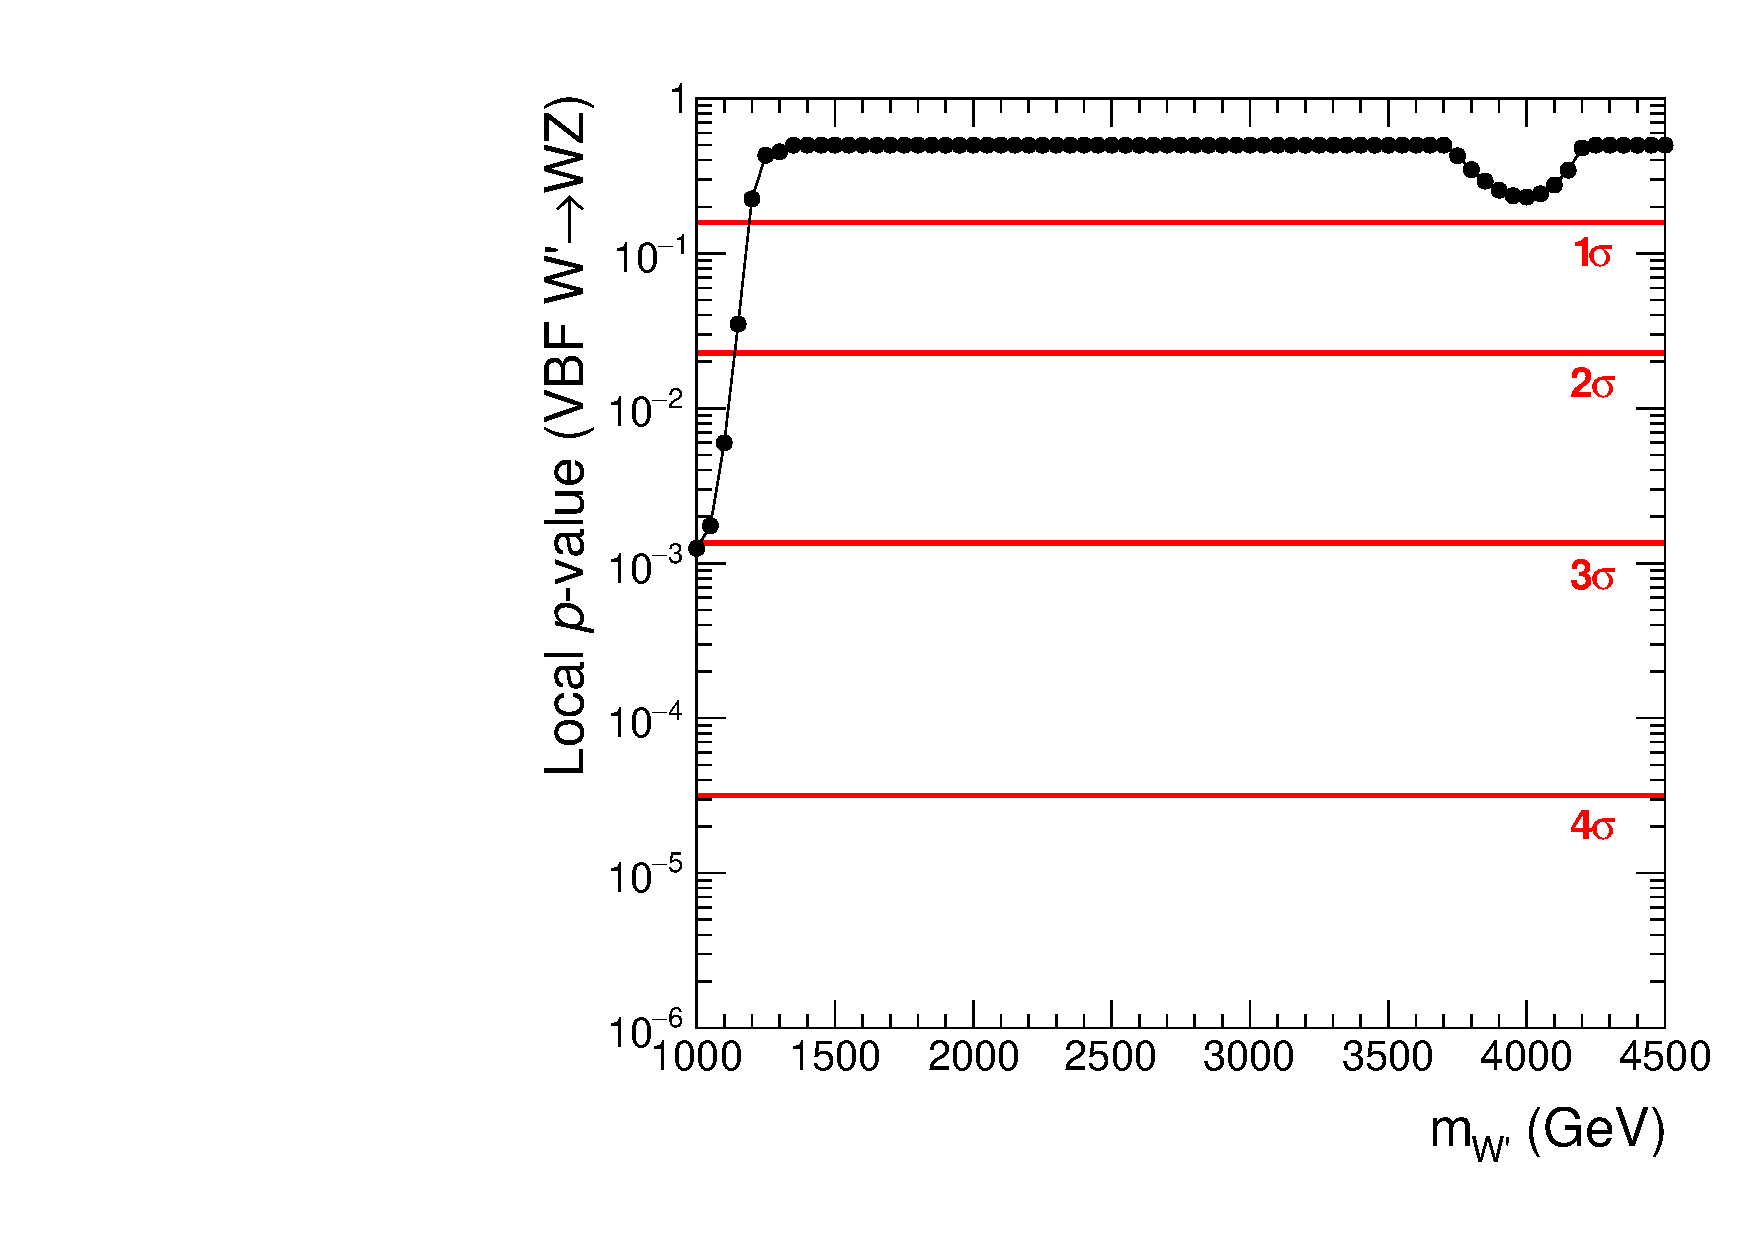
\includegraphics[width=0.33\textwidth]{fig/results/pvalue_VBFWprToWZ.pdf}\\
  \caption{
    Exclusion limits on the product of the production cross section with the branching ratio (left) and $p$-values (right) for a new charged spin-1 resonance produced via Drell-Yan (top row) and decaying to \WH, and for a new charged spin-1 resonance produced via Drell-Yan (middle row) or vector boson fusion (bottom row) and decaying to \WZ, as a function of the resonance mass hypothesis \MX, compared with the predicted cross sections for a \Wpr from HVT model B (for \DY) or HVT model C with $c_\mathrm{H}=3$ (for \VBF).
    The signal cross section uncertainties are shown as red cross-hatched bands.
  }
  \label{fig:limits_pvalue_spin1_char}
\end{figure}

\begin{figure}[htbp]
  \centering
  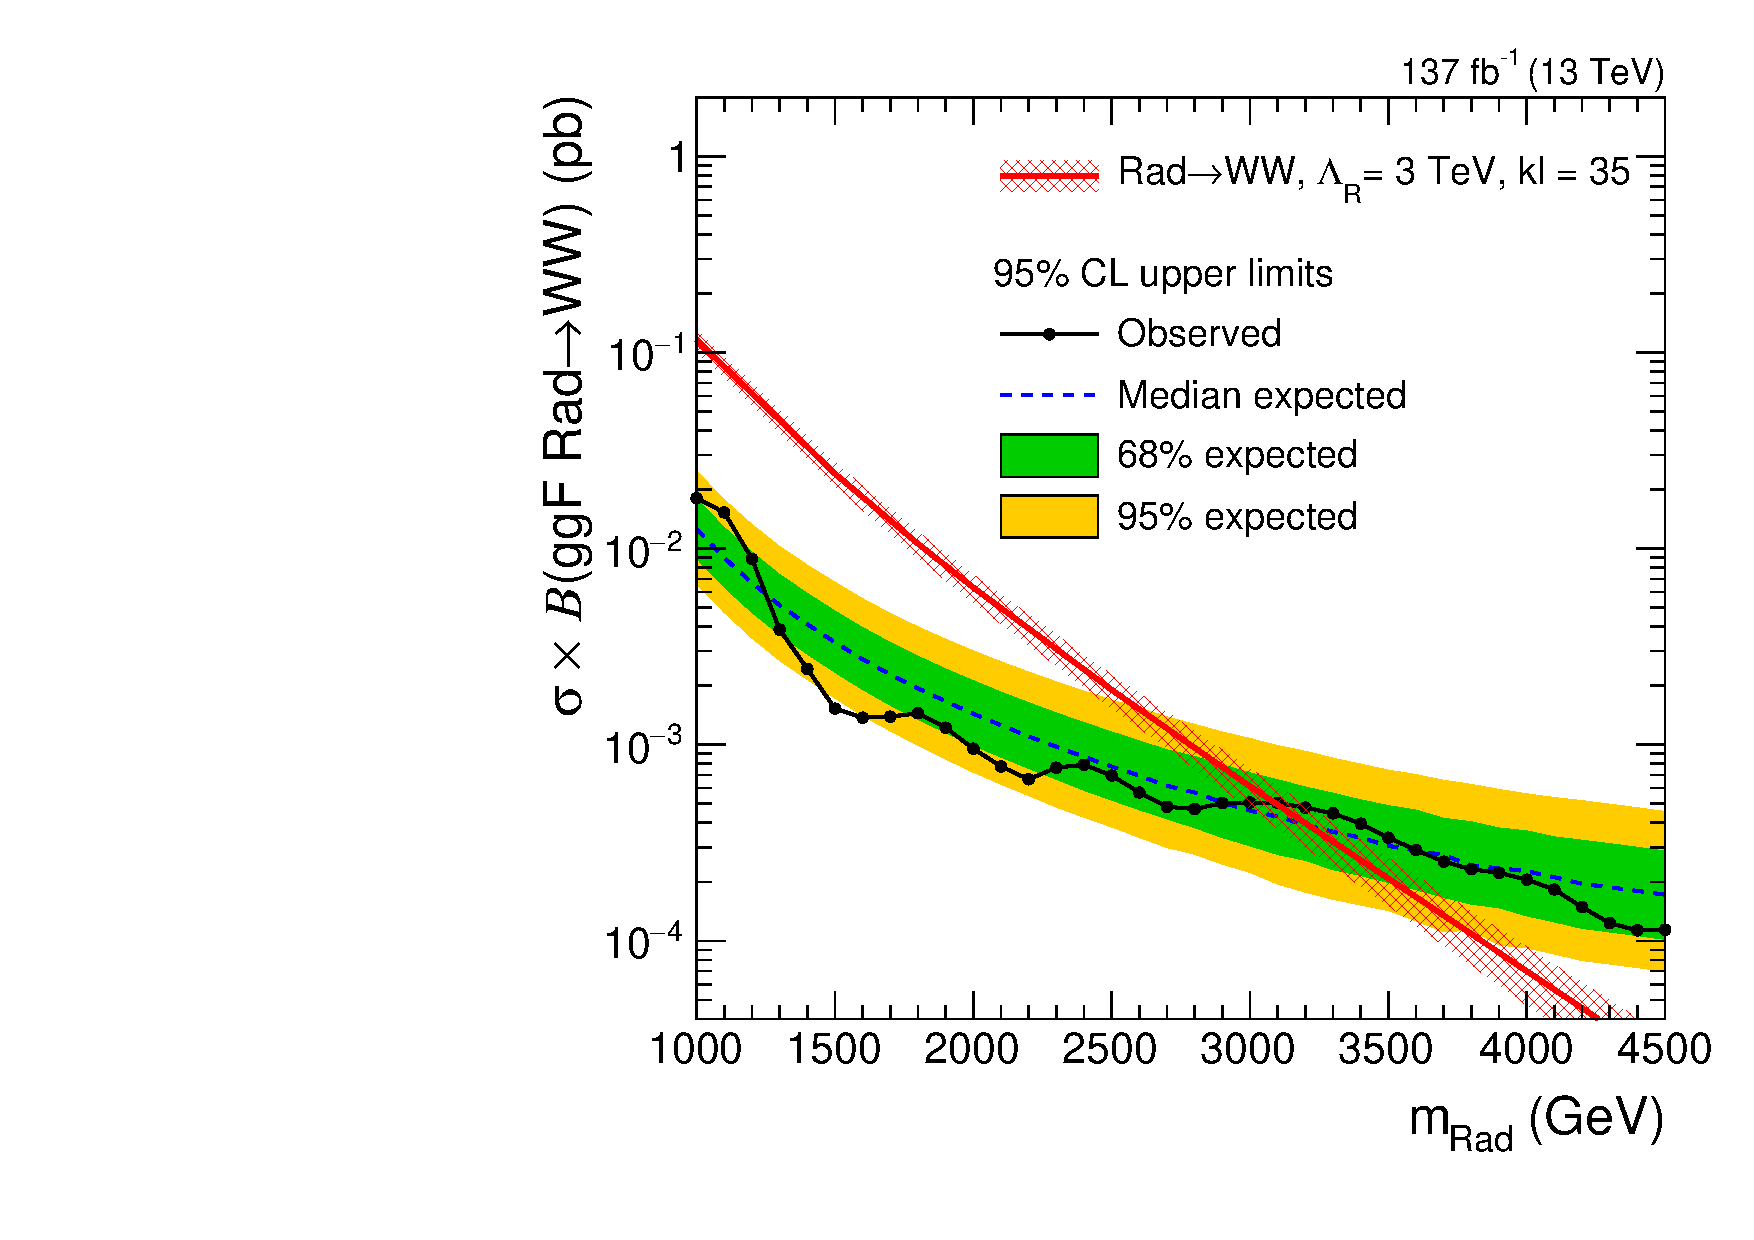
\includegraphics[width=0.33\textwidth]{fig/results/limits_RadToWW.pdf}
  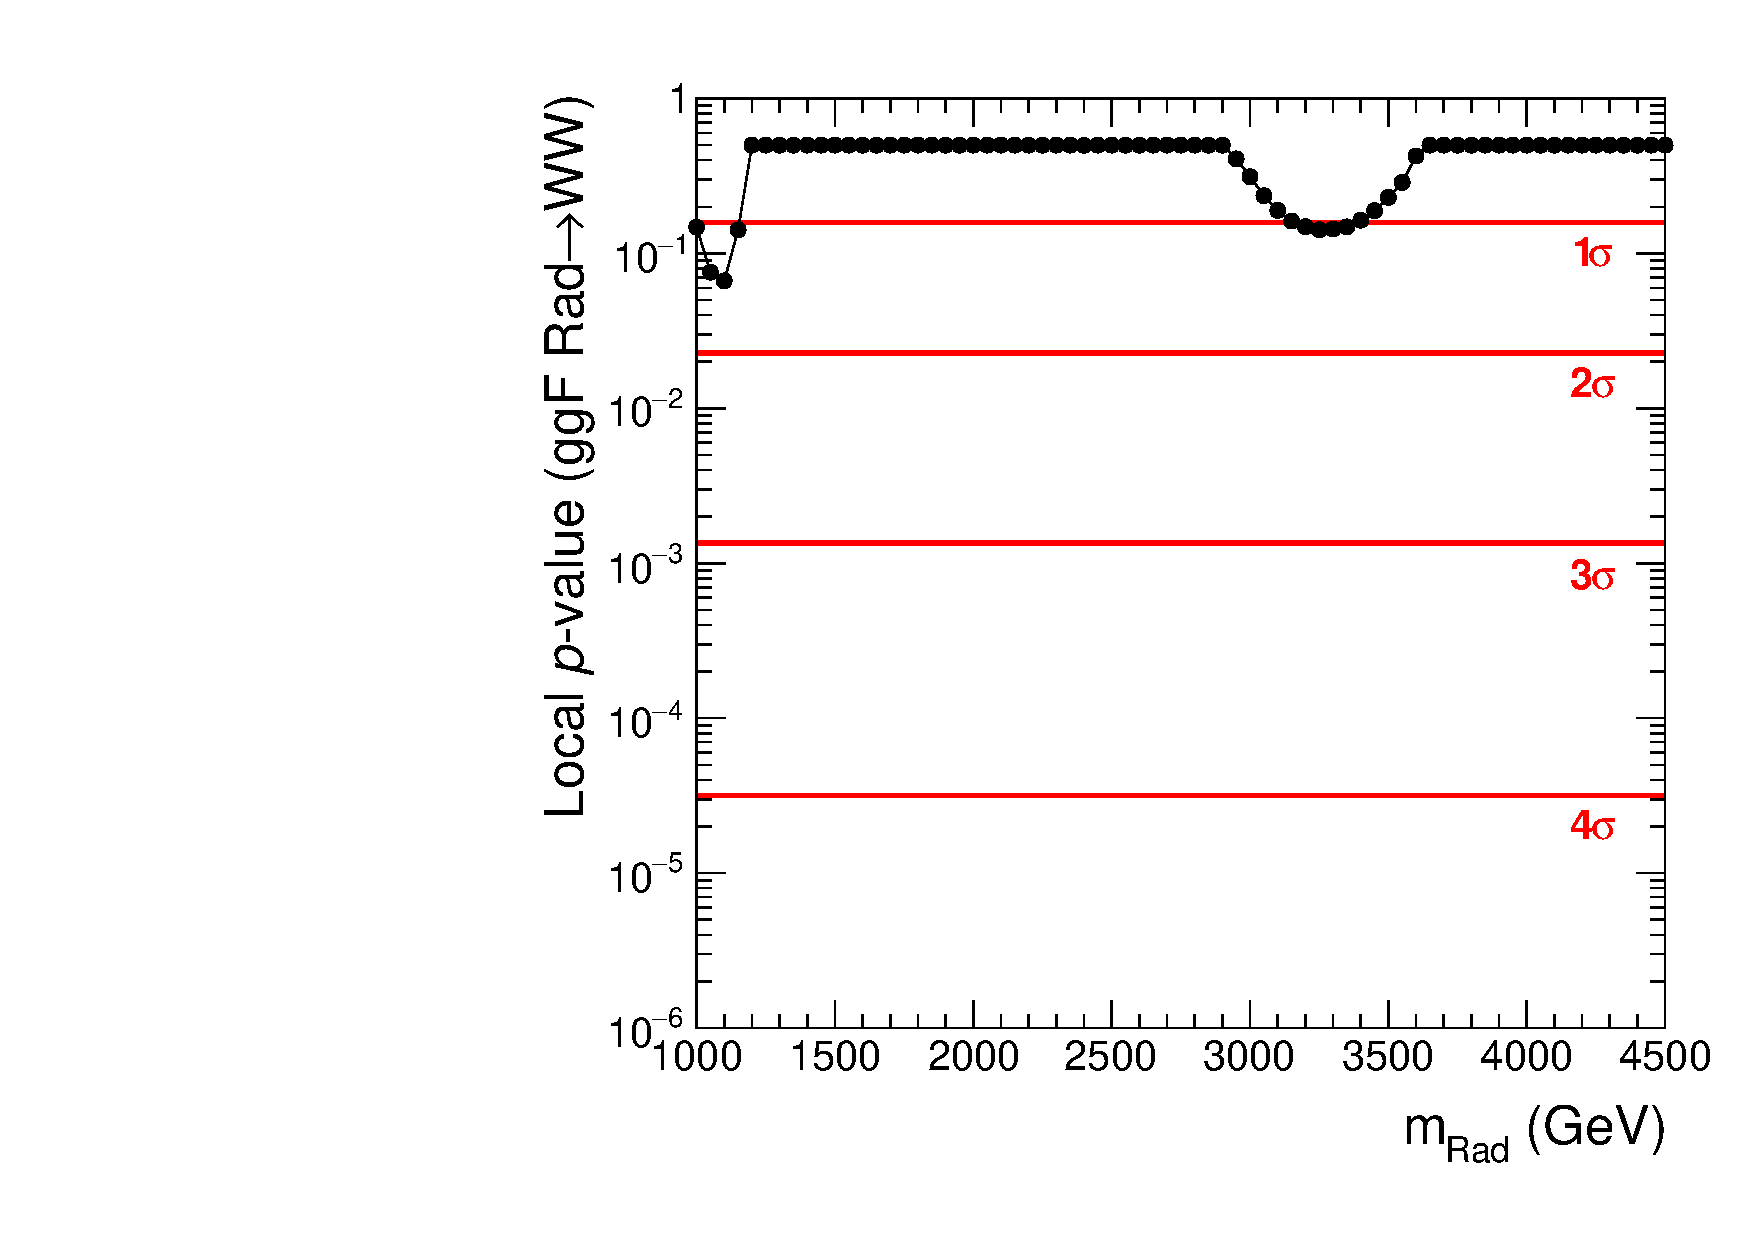
\includegraphics[width=0.33\textwidth]{fig/results/pvalue_RadToWW.pdf}\\
  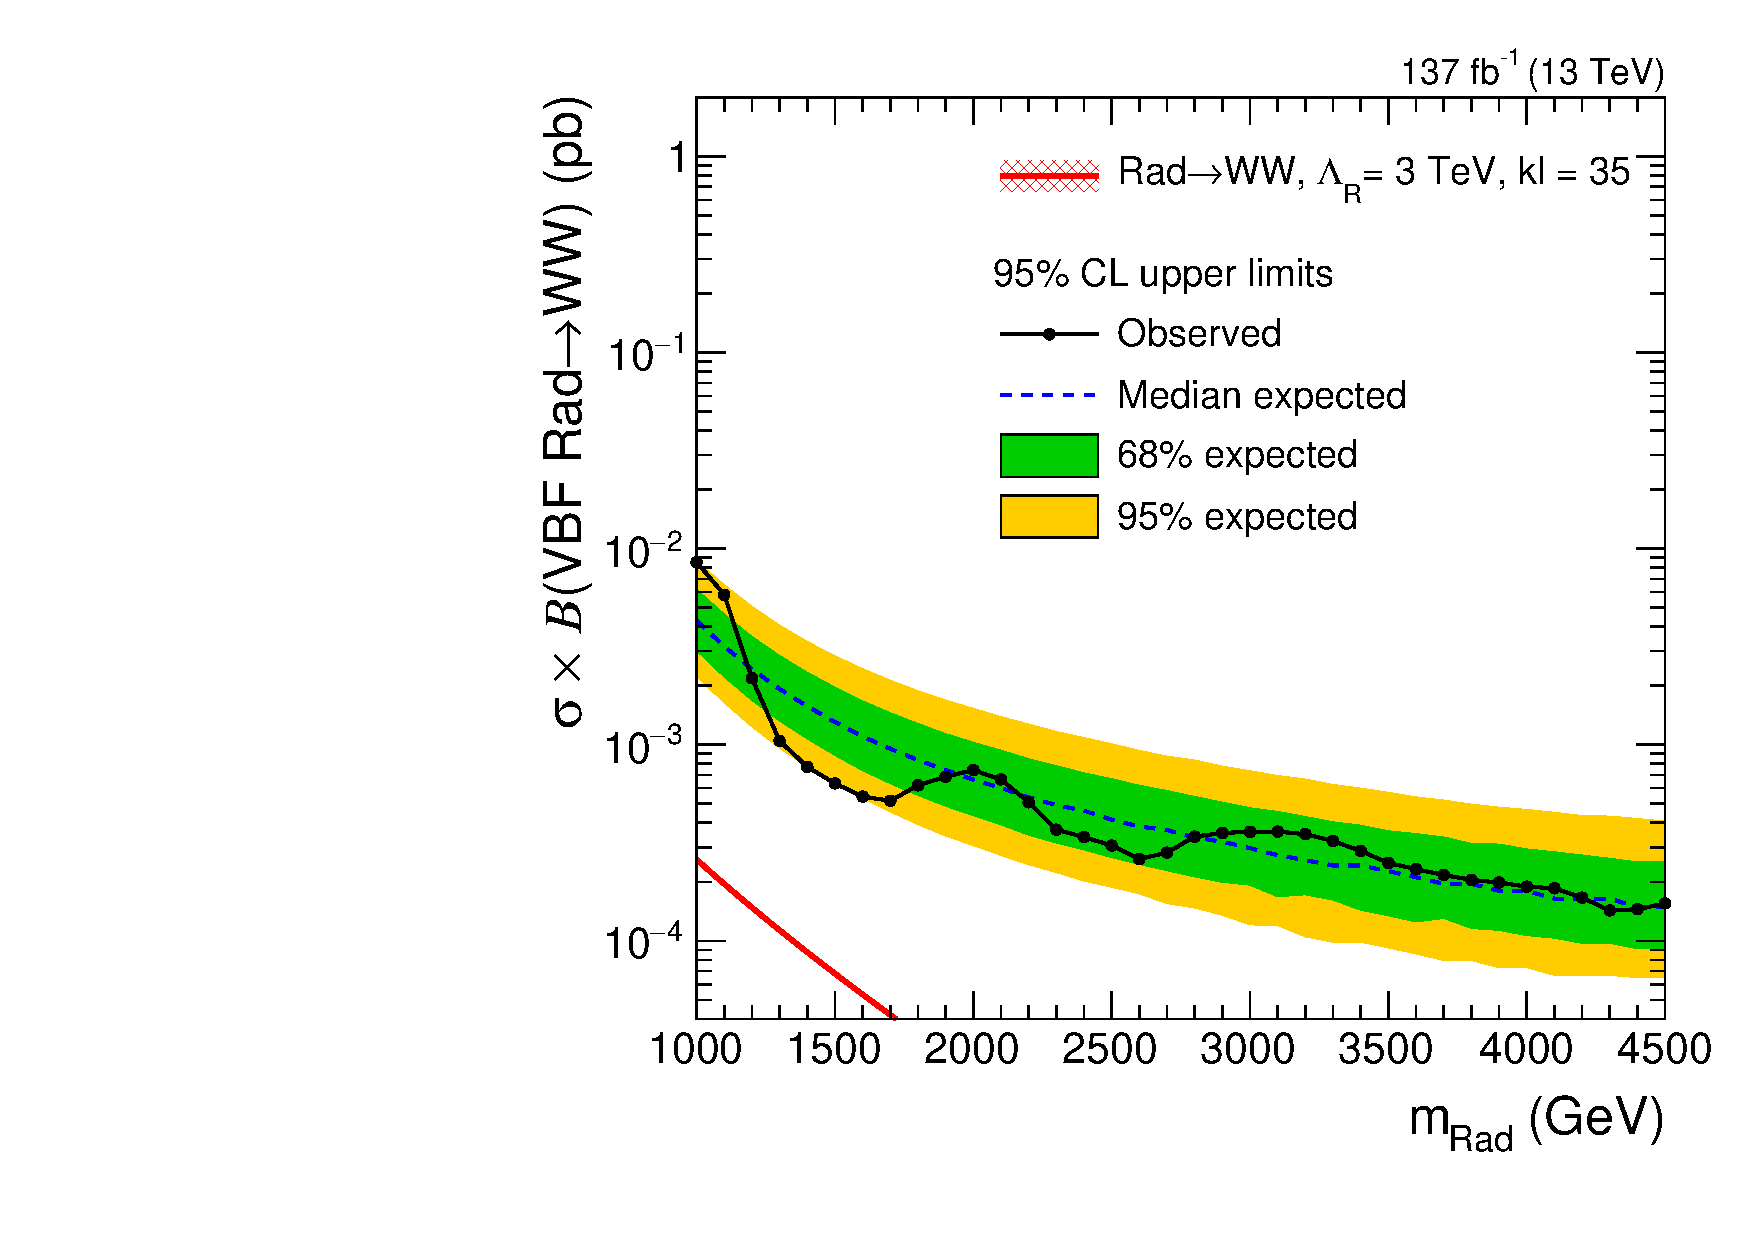
\includegraphics[width=0.33\textwidth]{fig/results/limits_VBFRadToWW.pdf}
  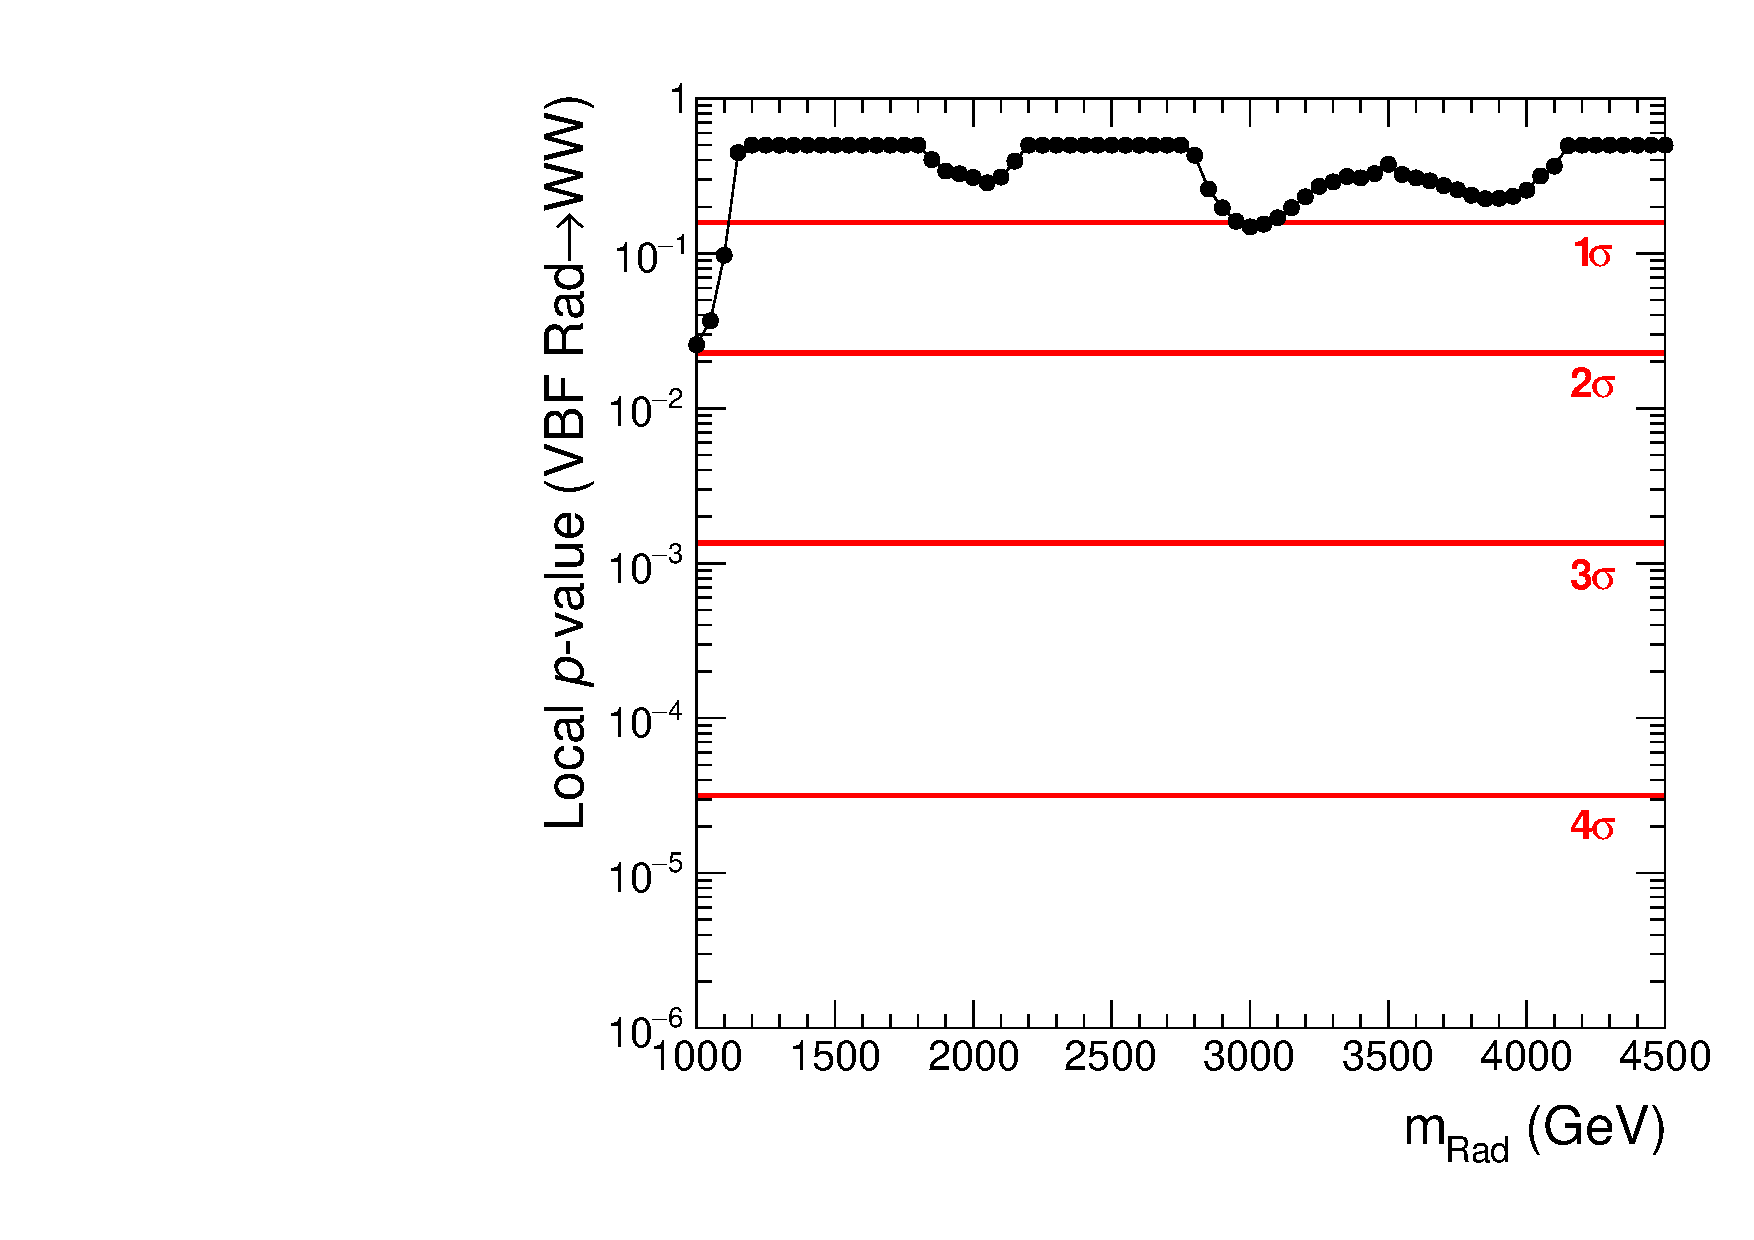
\includegraphics[width=0.33\textwidth]{fig/results/pvalue_VBFRadToWW.pdf}\\
  \caption{
    Exclusion limits on the product of the production cross section with the branching ratio (left) and $p$-values (right) for a new neutral spin-2 resonance produced via gluon-gluon fusion (top row) or vector boson fusion (bottom row) and decaying to \WW, as a function of the resonance mass hypothesis \MX, compared with the predicted cross sections for a \GBulk with curvature $\tilde{k}=0.5$.
    The signal cross section uncertainties are shown as red cross-hatched bands.
  }
  \label{fig:limits_pvalue_spin2}
\end{figure}
